% Options for packages loaded elsewhere
\PassOptionsToPackage{unicode}{hyperref}
\PassOptionsToPackage{hyphens}{url}
\PassOptionsToPackage{dvipsnames,svgnames,x11names}{xcolor}
%
\documentclass[
  letterpaper,
  DIV=11,
  numbers=noendperiod]{scrartcl}

\usepackage{amsmath,amssymb}
\usepackage{lmodern}
\usepackage{iftex}
\ifPDFTeX
  \usepackage[T1]{fontenc}
  \usepackage[utf8]{inputenc}
  \usepackage{textcomp} % provide euro and other symbols
\else % if luatex or xetex
  \usepackage{unicode-math}
  \defaultfontfeatures{Scale=MatchLowercase}
  \defaultfontfeatures[\rmfamily]{Ligatures=TeX,Scale=1}
\fi
% Use upquote if available, for straight quotes in verbatim environments
\IfFileExists{upquote.sty}{\usepackage{upquote}}{}
\IfFileExists{microtype.sty}{% use microtype if available
  \usepackage[]{microtype}
  \UseMicrotypeSet[protrusion]{basicmath} % disable protrusion for tt fonts
}{}
\makeatletter
\@ifundefined{KOMAClassName}{% if non-KOMA class
  \IfFileExists{parskip.sty}{%
    \usepackage{parskip}
  }{% else
    \setlength{\parindent}{0pt}
    \setlength{\parskip}{6pt plus 2pt minus 1pt}}
}{% if KOMA class
  \KOMAoptions{parskip=half}}
\makeatother
\usepackage{xcolor}
\setlength{\emergencystretch}{3em} % prevent overfull lines
\setcounter{secnumdepth}{-\maxdimen} % remove section numbering
% Make \paragraph and \subparagraph free-standing
\ifx\paragraph\undefined\else
  \let\oldparagraph\paragraph
  \renewcommand{\paragraph}[1]{\oldparagraph{#1}\mbox{}}
\fi
\ifx\subparagraph\undefined\else
  \let\oldsubparagraph\subparagraph
  \renewcommand{\subparagraph}[1]{\oldsubparagraph{#1}\mbox{}}
\fi

\usepackage{color}
\usepackage{fancyvrb}
\newcommand{\VerbBar}{|}
\newcommand{\VERB}{\Verb[commandchars=\\\{\}]}
\DefineVerbatimEnvironment{Highlighting}{Verbatim}{commandchars=\\\{\}}
% Add ',fontsize=\small' for more characters per line
\usepackage{framed}
\definecolor{shadecolor}{RGB}{241,243,245}
\newenvironment{Shaded}{\begin{snugshade}}{\end{snugshade}}
\newcommand{\AlertTok}[1]{\textcolor[rgb]{0.68,0.00,0.00}{#1}}
\newcommand{\AnnotationTok}[1]{\textcolor[rgb]{0.37,0.37,0.37}{#1}}
\newcommand{\AttributeTok}[1]{\textcolor[rgb]{0.40,0.45,0.13}{#1}}
\newcommand{\BaseNTok}[1]{\textcolor[rgb]{0.68,0.00,0.00}{#1}}
\newcommand{\BuiltInTok}[1]{\textcolor[rgb]{0.00,0.23,0.31}{#1}}
\newcommand{\CharTok}[1]{\textcolor[rgb]{0.13,0.47,0.30}{#1}}
\newcommand{\CommentTok}[1]{\textcolor[rgb]{0.37,0.37,0.37}{#1}}
\newcommand{\CommentVarTok}[1]{\textcolor[rgb]{0.37,0.37,0.37}{\textit{#1}}}
\newcommand{\ConstantTok}[1]{\textcolor[rgb]{0.56,0.35,0.01}{#1}}
\newcommand{\ControlFlowTok}[1]{\textcolor[rgb]{0.00,0.23,0.31}{#1}}
\newcommand{\DataTypeTok}[1]{\textcolor[rgb]{0.68,0.00,0.00}{#1}}
\newcommand{\DecValTok}[1]{\textcolor[rgb]{0.68,0.00,0.00}{#1}}
\newcommand{\DocumentationTok}[1]{\textcolor[rgb]{0.37,0.37,0.37}{\textit{#1}}}
\newcommand{\ErrorTok}[1]{\textcolor[rgb]{0.68,0.00,0.00}{#1}}
\newcommand{\ExtensionTok}[1]{\textcolor[rgb]{0.00,0.23,0.31}{#1}}
\newcommand{\FloatTok}[1]{\textcolor[rgb]{0.68,0.00,0.00}{#1}}
\newcommand{\FunctionTok}[1]{\textcolor[rgb]{0.28,0.35,0.67}{#1}}
\newcommand{\ImportTok}[1]{\textcolor[rgb]{0.00,0.46,0.62}{#1}}
\newcommand{\InformationTok}[1]{\textcolor[rgb]{0.37,0.37,0.37}{#1}}
\newcommand{\KeywordTok}[1]{\textcolor[rgb]{0.00,0.23,0.31}{#1}}
\newcommand{\NormalTok}[1]{\textcolor[rgb]{0.00,0.23,0.31}{#1}}
\newcommand{\OperatorTok}[1]{\textcolor[rgb]{0.37,0.37,0.37}{#1}}
\newcommand{\OtherTok}[1]{\textcolor[rgb]{0.00,0.23,0.31}{#1}}
\newcommand{\PreprocessorTok}[1]{\textcolor[rgb]{0.68,0.00,0.00}{#1}}
\newcommand{\RegionMarkerTok}[1]{\textcolor[rgb]{0.00,0.23,0.31}{#1}}
\newcommand{\SpecialCharTok}[1]{\textcolor[rgb]{0.37,0.37,0.37}{#1}}
\newcommand{\SpecialStringTok}[1]{\textcolor[rgb]{0.13,0.47,0.30}{#1}}
\newcommand{\StringTok}[1]{\textcolor[rgb]{0.13,0.47,0.30}{#1}}
\newcommand{\VariableTok}[1]{\textcolor[rgb]{0.07,0.07,0.07}{#1}}
\newcommand{\VerbatimStringTok}[1]{\textcolor[rgb]{0.13,0.47,0.30}{#1}}
\newcommand{\WarningTok}[1]{\textcolor[rgb]{0.37,0.37,0.37}{\textit{#1}}}

\providecommand{\tightlist}{%
  \setlength{\itemsep}{0pt}\setlength{\parskip}{0pt}}\usepackage{longtable,booktabs,array}
\usepackage{calc} % for calculating minipage widths
% Correct order of tables after \paragraph or \subparagraph
\usepackage{etoolbox}
\makeatletter
\patchcmd\longtable{\par}{\if@noskipsec\mbox{}\fi\par}{}{}
\makeatother
% Allow footnotes in longtable head/foot
\IfFileExists{footnotehyper.sty}{\usepackage{footnotehyper}}{\usepackage{footnote}}
\makesavenoteenv{longtable}
\usepackage{graphicx}
\makeatletter
\def\maxwidth{\ifdim\Gin@nat@width>\linewidth\linewidth\else\Gin@nat@width\fi}
\def\maxheight{\ifdim\Gin@nat@height>\textheight\textheight\else\Gin@nat@height\fi}
\makeatother
% Scale images if necessary, so that they will not overflow the page
% margins by default, and it is still possible to overwrite the defaults
% using explicit options in \includegraphics[width, height, ...]{}
\setkeys{Gin}{width=\maxwidth,height=\maxheight,keepaspectratio}
% Set default figure placement to htbp
\makeatletter
\def\fps@figure{htbp}
\makeatother

\usepackage{booktabs}
\usepackage{longtable}
\usepackage{array}
\usepackage{multirow}
\usepackage{wrapfig}
\usepackage{float}
\usepackage{colortbl}
\usepackage{pdflscape}
\usepackage{tabu}
\usepackage{threeparttable}
\usepackage{threeparttablex}
\usepackage[normalem]{ulem}
\usepackage{makecell}
\usepackage{xcolor}
\KOMAoption{captions}{tableheading}
\makeatletter
\makeatother
\makeatletter
\makeatother
\makeatletter
\@ifpackageloaded{caption}{}{\usepackage{caption}}
\AtBeginDocument{%
\ifdefined\contentsname
  \renewcommand*\contentsname{Table of contents}
\else
  \newcommand\contentsname{Table of contents}
\fi
\ifdefined\listfigurename
  \renewcommand*\listfigurename{List of Figures}
\else
  \newcommand\listfigurename{List of Figures}
\fi
\ifdefined\listtablename
  \renewcommand*\listtablename{List of Tables}
\else
  \newcommand\listtablename{List of Tables}
\fi
\ifdefined\figurename
  \renewcommand*\figurename{Figure}
\else
  \newcommand\figurename{Figure}
\fi
\ifdefined\tablename
  \renewcommand*\tablename{Table}
\else
  \newcommand\tablename{Table}
\fi
}
\@ifpackageloaded{float}{}{\usepackage{float}}
\floatstyle{ruled}
\@ifundefined{c@chapter}{\newfloat{codelisting}{h}{lop}}{\newfloat{codelisting}{h}{lop}[chapter]}
\floatname{codelisting}{Listing}
\newcommand*\listoflistings{\listof{codelisting}{List of Listings}}
\makeatother
\makeatletter
\@ifpackageloaded{caption}{}{\usepackage{caption}}
\@ifpackageloaded{subcaption}{}{\usepackage{subcaption}}
\makeatother
\makeatletter
\@ifpackageloaded{tcolorbox}{}{\usepackage[many]{tcolorbox}}
\makeatother
\makeatletter
\@ifundefined{shadecolor}{\definecolor{shadecolor}{rgb}{.97, .97, .97}}
\makeatother
\makeatletter
\makeatother
\ifLuaTeX
  \usepackage{selnolig}  % disable illegal ligatures
\fi
\IfFileExists{bookmark.sty}{\usepackage{bookmark}}{\usepackage{hyperref}}
\IfFileExists{xurl.sty}{\usepackage{xurl}}{} % add URL line breaks if available
\urlstyle{same} % disable monospaced font for URLs
\hypersetup{
  pdftitle={Analysing used car sales data for Pakistan},
  colorlinks=true,
  linkcolor={blue},
  filecolor={Maroon},
  citecolor={Blue},
  urlcolor={Blue},
  pdfcreator={LaTeX via pandoc}}

\title{Analysing used car sales data for Pakistan}
\usepackage{etoolbox}
\makeatletter
\providecommand{\subtitle}[1]{% add subtitle to \maketitle
  \apptocmd{\@title}{\par {\large #1 \par}}{}{}
}
\makeatother
\subtitle{Zahid Asghar, SOE, QAU}
\author{}
\date{}

\begin{document}
\maketitle
\ifdefined\Shaded\renewenvironment{Shaded}{\begin{tcolorbox}[boxrule=0pt, colback={shadecolor}, breakable, enhanced, frame hidden]}{\end{tcolorbox}}\fi

\renewcommand*\contentsname{Table of contents}
{
\hypersetup{linkcolor=}
\setcounter{tocdepth}{3}
\tableofcontents
}
\hypertarget{section}{%
\subsection{}\label{section}}

\hypertarget{section-1}{%
\subsubsection{\texorpdfstring{{}}{}}\label{section-1}}

{zasghar@qau.edu.pk zahedasghar zahidasghar.com}

\begin{Shaded}
\begin{Highlighting}[]
\FunctionTok{library}\NormalTok{(tidyverse)}
\FunctionTok{library}\NormalTok{(gapminder)}
\FunctionTok{library}\NormalTok{(kableExtra)}
\FunctionTok{library}\NormalTok{(patchwork)}
\FunctionTok{library}\NormalTok{(fontawesome)}
\FunctionTok{library}\NormalTok{(gapminder)}
\FunctionTok{library}\NormalTok{(scales)}
\FunctionTok{library}\NormalTok{(httr)}
\NormalTok{clrs }\OtherTok{\textless{}{-}}\NormalTok{ MetBrewer}\SpecialCharTok{::}\FunctionTok{met.brewer}\NormalTok{(}\AttributeTok{name =} \StringTok{"Java"}\NormalTok{)}
\NormalTok{clrs\_lt }\OtherTok{\textless{}{-}}\NormalTok{ colorspace}\SpecialCharTok{::}\FunctionTok{lighten}\NormalTok{(clrs, }\FloatTok{0.9}\NormalTok{)}
\NormalTok{knitr}\SpecialCharTok{::}\NormalTok{opts\_chunk}\SpecialCharTok{$}\FunctionTok{set}\NormalTok{(}\AttributeTok{fig.retina =} \DecValTok{3}\NormalTok{, }\AttributeTok{collapse =} \ConstantTok{TRUE}\NormalTok{)}
\FunctionTok{options}\NormalTok{(}\AttributeTok{digits =} \DecValTok{3}\NormalTok{, }\AttributeTok{width =} \DecValTok{75}\NormalTok{)}
\end{Highlighting}
\end{Shaded}

\hypertarget{why-r}{%
\section{Why R}\label{why-r}}

There is an increasing recognition of reproducibility of research,
though it has limited recognition in social sciences. The document in
your hand is written in \texttt{Quarto}. \texttt{Quarto} which can be
used for pdf, html, word, PowerPoint/Slidy/Beamer Presentations,
Webpages, LaTex and many others. Besides learning basics of R-coding,
another objective of this workshop is understanding the importance of
reproducibility. Building this new habit of reproducible work at times
maybe little challenging occasionally. Getting rid of culture of copying
and pasting, and sparing this time for doing data analysis and research
is one of the objectives of this or coming workshops. Purpose is to help
you to get away from this tedious activity so that you can spend more
time \textbf{doing science}.

\hypertarget{installing-and-loading-packages}{%
\subsection{Installing and loading
packages}\label{installing-and-loading-packages}}

The first thing we need to do is install and then load the
\texttt{tidyverse} set of R packages to provide us with lots of extra
functionality. You only need to install this once: once it's installed
we can simply load it into the workspace using the library() function
each time we open a new R session.

Understanding data sets requires many hours/days or in some cases
weeks.There are many commercially available software but open source
community based software have now dominated and R is one of these. R
makes data understanding process as easy as possible through the
\texttt{dplyr} package. It is one of the easiest solution for code-based
data analysis. We will learn in this training how to do it. In case, you
need more information, you can watch my
\href{https://youtu.be/ZNBZevfYgo0}{videos}.

I have discussed the
\href{https://cran.r-project.org/web/packages/gapminder/index.html}{Gapminder
dataset} in \href{youtube}{my videos}, you can watch those videos.
\texttt{gapminder} package is available through CRAN, so make sure to
install it. Here's how to load in all required packages:

\begin{Shaded}
\begin{Highlighting}[]
\FunctionTok{library}\NormalTok{(tidyverse)}
\FunctionTok{library}\NormalTok{(knitr)}
\FunctionTok{library}\NormalTok{(kableExtra)}
\CommentTok{\#install.packages("gapminder")}
\FunctionTok{library}\NormalTok{(hrbrthemes)}
\FunctionTok{library}\NormalTok{(viridis)}
\FunctionTok{library}\NormalTok{(kableExtra)}
\FunctionTok{options}\NormalTok{(}\AttributeTok{knitr.table.format =} \StringTok{"html"}\NormalTok{)}
\FunctionTok{library}\NormalTok{(plotly)}
\FunctionTok{library}\NormalTok{(gridExtra)}
\FunctionTok{library}\NormalTok{(ggrepel)}
\end{Highlighting}
\end{Shaded}

**The dataset to be used is pakwheels data obtained from kaggle and you
can download data from the link
\href{https://www.kaggle.com/datasets/spideysloth/pakwheels-cars-dataset}{data
download} or from my github repository. We read \texttt{data} as follows

\begin{Shaded}
\begin{Highlighting}[]
\CommentTok{\#pakwheels\_11Jul2020 \textless{}{-} read\_csv("C:/Users/92300/Downloads/archive/pakwheels{-}11Jul2020.csv")}
\CommentTok{\#pakwheels\textless{}{-}saveRDS(pakwheels\_11Jul2020,file = "pakwheels.rds")}

\NormalTok{pakwheels }\OtherTok{\textless{}{-}} \FunctionTok{readRDS}\NormalTok{(}\StringTok{"D:/RepTemplates/data\_analytics/pakwheels.rds"}\NormalTok{)}

\NormalTok{pakwheels}
\DocumentationTok{\#\# \# A tibble: 56,186 x 16}
\DocumentationTok{\#\#    \textasciigrave{}Ad No\textasciigrave{} Name       Price Model\textasciitilde{}1 Locat\textasciitilde{}2 Mileage Regis\textasciitilde{}3 Engin\textasciitilde{}4 Engin\textasciitilde{}5}
\DocumentationTok{\#\#      \textless{}dbl\textgreater{} \textless{}chr\textgreater{}      \textless{}chr\textgreater{}   \textless{}dbl\textgreater{} \textless{}chr\textgreater{}     \textless{}dbl\textgreater{} \textless{}chr\textgreater{}   \textless{}chr\textgreater{}   \textless{}chr\textgreater{}  }
\DocumentationTok{\#\#  1 4096758 Toyota Vi\textasciitilde{} 2385\textasciitilde{}    2017 G{-} 8, \textasciitilde{}    9869 Un{-}Reg\textasciitilde{} Petrol  1000 cc}
\DocumentationTok{\#\#  2 4168305 Toyota Co\textasciitilde{} 1110\textasciitilde{}    2019 Peshaw\textasciitilde{}   11111 Islama\textasciitilde{} Petrol  1300 cc}
\DocumentationTok{\#\#  3 4168298 Suzuki Al\textasciitilde{} 1530\textasciitilde{}    2019 Akora \textasciitilde{}   17500 Un{-}Reg\textasciitilde{} Petrol  660 cc }
\DocumentationTok{\#\#  4 4168307 Suzuki Al\textasciitilde{} 1650\textasciitilde{}    2019 Abdull\textasciitilde{}    9600 Lahore  Petrol  660 cc }
\DocumentationTok{\#\#  5 4168306 Toyota Co\textasciitilde{} 1435\textasciitilde{}    2010 9th Av\textasciitilde{}  120000 Islama\textasciitilde{} Petrol  1300 cc}
\DocumentationTok{\#\#  6 4168303 Honda Civ\textasciitilde{} 3850\textasciitilde{}    2017 Peshaw\textasciitilde{}   22000 Islama\textasciitilde{} Petrol  1500 cc}
\DocumentationTok{\#\#  7 4168304 Suzuki Wa\textasciitilde{} 1440\textasciitilde{}    2017 Gulber\textasciitilde{}   31000 Lahore  Petrol  1000 cc}
\DocumentationTok{\#\#  8 4168309 Mitsubish\textasciitilde{} 1425\textasciitilde{}    2012 Askari\textasciitilde{}  101000 Lahore  Petrol  1000 cc}
\DocumentationTok{\#\#  9 4168310 Toyota Pr\textasciitilde{} 2650\textasciitilde{}    1998 Sargod\textasciitilde{}  110000 Rawalp\textasciitilde{} Diesel  3000 cc}
\DocumentationTok{\#\# 10 4168311 Honda Civ\textasciitilde{} 3350\textasciitilde{}    2017 Air Av\textasciitilde{}   60000 Lahore  Petrol  1800 cc}
\DocumentationTok{\#\# \# ... with 56,176 more rows, 7 more variables: Transmission \textless{}chr\textgreater{},}
\DocumentationTok{\#\# \#   Color \textless{}chr\textgreater{}, Assembly \textless{}chr\textgreater{}, \textasciigrave{}Body Type\textasciigrave{} \textless{}chr\textgreater{}, Features \textless{}chr\textgreater{},}
\DocumentationTok{\#\# \#   \textasciigrave{}Last Updated\textasciigrave{} \textless{}chr\textgreater{}, URL \textless{}chr\textgreater{}, and abbreviated variable names}
\DocumentationTok{\#\# \#   1: \textasciigrave{}Model Year\textasciigrave{}, 2: Location, 3: \textasciigrave{}Registered City\textasciigrave{}, 4: \textasciigrave{}Engine Type\textasciigrave{},}
\DocumentationTok{\#\# \#   5: \textasciigrave{}Engine Capacity\textasciigrave{}}
\end{Highlighting}
\end{Shaded}

First few rows of data are displayed here and there \texttt{56186}
observations in total. We will start from scratch and end up a
sophisticated analysis. Firs step in dealing with data is to clean up
the data and bringing it in workable format. It is said that every
\texttt{tidy} data is alike but every messy data is messy in its own
way. So lets see whether this data are in neat and clean format.

\hypertarget{data-overview}{%
\subsection{Data Overview}\label{data-overview}}

\textbf{Pipe operator} \texttt{\%\textgreater{}\%} or
\texttt{\textbar{}\textgreater{}} play very nicely with dplyr and make
our code very easy to understand. For this lets have an overview of data
for which one can use \texttt{glimpse()} or \texttt{str()} for structure
of data and to view entire spreadsheet use \texttt{View()}.\texttt{View}
command opens data in new worksheet while glimpse lists nature of
variables (numeric/character/factor\ldots) and total number of rows and
columns.To see first 6 and last 6 observations use \texttt{head()} and
\texttt{tail()} ,respectively.

\begin{Shaded}
\begin{Highlighting}[]

\NormalTok{pakwheels}\SpecialCharTok{|\textgreater{}}\FunctionTok{glimpse}\NormalTok{()}
\DocumentationTok{\#\# Rows: 56,186}
\DocumentationTok{\#\# Columns: 16}
\DocumentationTok{\#\# $ \textasciigrave{}Ad No\textasciigrave{}           \textless{}dbl\textgreater{} 4096758, 4168305, 4168298, 4168307, 4168306, 41\textasciitilde{}}
\DocumentationTok{\#\# $ Name              \textless{}chr\textgreater{} "Toyota Vitz F 1.0 2017", "Toyota Corolla GLi A\textasciitilde{}}
\DocumentationTok{\#\# $ Price             \textless{}chr\textgreater{} "2385000.0", "111000.00000000001", "1530000.0",\textasciitilde{}}
\DocumentationTok{\#\# $ \textasciigrave{}Model Year\textasciigrave{}      \textless{}dbl\textgreater{} 2017, 2019, 2019, 2019, 2010, 2017, 2017, 2012,\textasciitilde{}}
\DocumentationTok{\#\# $ Location          \textless{}chr\textgreater{} "G{-} 8, Islamabad Islamabad", "Peshawar KPK", "A\textasciitilde{}}
\DocumentationTok{\#\# $ Mileage           \textless{}dbl\textgreater{} 9869, 11111, 17500, 9600, 120000, 22000, 31000,\textasciitilde{}}
\DocumentationTok{\#\# $ \textasciigrave{}Registered City\textasciigrave{} \textless{}chr\textgreater{} "Un{-}Registered", "Islamabad", "Un{-}Registered", \textasciitilde{}}
\DocumentationTok{\#\# $ \textasciigrave{}Engine Type\textasciigrave{}     \textless{}chr\textgreater{} "Petrol", "Petrol", "Petrol", "Petrol", "Petrol\textasciitilde{}}
\DocumentationTok{\#\# $ \textasciigrave{}Engine Capacity\textasciigrave{} \textless{}chr\textgreater{} "1000 cc", "1300 cc", "660 cc", "660 cc", "1300\textasciitilde{}}
\DocumentationTok{\#\# $ Transmission      \textless{}chr\textgreater{} "Automatic", "Automatic", "Automatic", "Manual"\textasciitilde{}}
\DocumentationTok{\#\# $ Color             \textless{}chr\textgreater{} "Silver", "White", "White", "White", "Black", "\textasciitilde{}}
\DocumentationTok{\#\# $ Assembly          \textless{}chr\textgreater{} "Imported", "Local", "Local", "Local", "Local",\textasciitilde{}}
\DocumentationTok{\#\# $ \textasciigrave{}Body Type\textasciigrave{}       \textless{}chr\textgreater{} "Hatchback", "Sedan", "Hatchback", "Hatchback",\textasciitilde{}}
\DocumentationTok{\#\# $ Features          \textless{}chr\textgreater{} "ABS, AM/FM Radio, Air Bags, Air Conditioning, \textasciitilde{}}
\DocumentationTok{\#\# $ \textasciigrave{}Last Updated\textasciigrave{}    \textless{}chr\textgreater{} "Jul 11, 2020", "Jul 12, 2020", "Jul 12, 2020",\textasciitilde{}}
\DocumentationTok{\#\# $ URL               \textless{}chr\textgreater{} "https://www.pakwheels.com/used{-}cars/toyota{-}vit\textasciitilde{}}
\FunctionTok{head}\NormalTok{(pakwheels)}
\DocumentationTok{\#\# \# A tibble: 6 x 16}
\DocumentationTok{\#\#   \textasciigrave{}Ad No\textasciigrave{} Name        Price Model\textasciitilde{}1 Locat\textasciitilde{}2 Mileage Regis\textasciitilde{}3 Engin\textasciitilde{}4 Engin\textasciitilde{}5}
\DocumentationTok{\#\#     \textless{}dbl\textgreater{} \textless{}chr\textgreater{}       \textless{}chr\textgreater{}   \textless{}dbl\textgreater{} \textless{}chr\textgreater{}     \textless{}dbl\textgreater{} \textless{}chr\textgreater{}   \textless{}chr\textgreater{}   \textless{}chr\textgreater{}  }
\DocumentationTok{\#\# 1 4096758 Toyota Vit\textasciitilde{} 2385\textasciitilde{}    2017 G{-} 8, \textasciitilde{}    9869 Un{-}Reg\textasciitilde{} Petrol  1000 cc}
\DocumentationTok{\#\# 2 4168305 Toyota Cor\textasciitilde{} 1110\textasciitilde{}    2019 Peshaw\textasciitilde{}   11111 Islama\textasciitilde{} Petrol  1300 cc}
\DocumentationTok{\#\# 3 4168298 Suzuki Alt\textasciitilde{} 1530\textasciitilde{}    2019 Akora \textasciitilde{}   17500 Un{-}Reg\textasciitilde{} Petrol  660 cc }
\DocumentationTok{\#\# 4 4168307 Suzuki Alt\textasciitilde{} 1650\textasciitilde{}    2019 Abdull\textasciitilde{}    9600 Lahore  Petrol  660 cc }
\DocumentationTok{\#\# 5 4168306 Toyota Cor\textasciitilde{} 1435\textasciitilde{}    2010 9th Av\textasciitilde{}  120000 Islama\textasciitilde{} Petrol  1300 cc}
\DocumentationTok{\#\# 6 4168303 Honda Civi\textasciitilde{} 3850\textasciitilde{}    2017 Peshaw\textasciitilde{}   22000 Islama\textasciitilde{} Petrol  1500 cc}
\DocumentationTok{\#\# \# ... with 7 more variables: Transmission \textless{}chr\textgreater{}, Color \textless{}chr\textgreater{},}
\DocumentationTok{\#\# \#   Assembly \textless{}chr\textgreater{}, \textasciigrave{}Body Type\textasciigrave{} \textless{}chr\textgreater{}, Features \textless{}chr\textgreater{},}
\DocumentationTok{\#\# \#   \textasciigrave{}Last Updated\textasciigrave{} \textless{}chr\textgreater{}, URL \textless{}chr\textgreater{}, and abbreviated variable names}
\DocumentationTok{\#\# \#   1: \textasciigrave{}Model Year\textasciigrave{}, 2: Location, 3: \textasciigrave{}Registered City\textasciigrave{}, 4: \textasciigrave{}Engine Type\textasciigrave{},}
\DocumentationTok{\#\# \#   5: \textasciigrave{}Engine Capacity\textasciigrave{}}
\FunctionTok{tail}\NormalTok{(pakwheels)}
\DocumentationTok{\#\# \# A tibble: 6 x 16}
\DocumentationTok{\#\#   \textasciigrave{}Ad No\textasciigrave{} Name        Price Model\textasciitilde{}1 Locat\textasciitilde{}2 Mileage Regis\textasciitilde{}3 Engin\textasciitilde{}4 Engin\textasciitilde{}5}
\DocumentationTok{\#\#     \textless{}dbl\textgreater{} \textless{}chr\textgreater{}       \textless{}chr\textgreater{}   \textless{}dbl\textgreater{} \textless{}chr\textgreater{}     \textless{}dbl\textgreater{} \textless{}chr\textgreater{}   \textless{}chr\textgreater{}   \textless{}chr\textgreater{}  }
\DocumentationTok{\#\# 1 3339018 Nissan Kix\textasciitilde{} 1900\textasciitilde{}    2012 Faisal\textasciitilde{}   42000 Faisal\textasciitilde{} Petrol  660 cc }
\DocumentationTok{\#\# 2 3349017 Honda Civi\textasciitilde{} 3250\textasciitilde{}    2015 Lahore\textasciitilde{}  125000 Lahore  Petrol  1800 cc}
\DocumentationTok{\#\# 3 3722322 Toyota Pri\textasciitilde{} 4000\textasciitilde{}    2015 Peshaw\textasciitilde{}   35000 Lahore  Hybrid  1800 cc}
\DocumentationTok{\#\# 4 3748215 Toyota Aqu\textasciitilde{} 3000\textasciitilde{}    2016 Gujran\textasciitilde{}   60000 Lahore  Petrol  1500 cc}
\DocumentationTok{\#\# 5 3785520 Honda Veze\textasciitilde{} Call\textasciitilde{}    2015 Multan\textasciitilde{}   45000 Un{-}Reg\textasciitilde{} Hybrid  1500 cc}
\DocumentationTok{\#\# 6 3806951 Toyota Cor\textasciitilde{} 2250\textasciitilde{}    2015 Gujran\textasciitilde{}   77000 Gujran\textasciitilde{} Petrol  1300 cc}
\DocumentationTok{\#\# \# ... with 7 more variables: Transmission \textless{}chr\textgreater{}, Color \textless{}chr\textgreater{},}
\DocumentationTok{\#\# \#   Assembly \textless{}chr\textgreater{}, \textasciigrave{}Body Type\textasciigrave{} \textless{}chr\textgreater{}, Features \textless{}chr\textgreater{},}
\DocumentationTok{\#\# \#   \textasciigrave{}Last Updated\textasciigrave{} \textless{}chr\textgreater{}, URL \textless{}chr\textgreater{}, and abbreviated variable names}
\DocumentationTok{\#\# \#   1: \textasciigrave{}Model Year\textasciigrave{}, 2: Location, 3: \textasciigrave{}Registered City\textasciigrave{}, 4: \textasciigrave{}Engine Type\textasciigrave{},}
\DocumentationTok{\#\# \#   5: \textasciigrave{}Engine Capacity\textasciigrave{}}
\end{Highlighting}
\end{Shaded}

One can observe that \texttt{Price} and \texttt{Engine\ Capacity} are
character variables while we know Price is numeric variable and should
fall in cateogry of \texttt{dbl} used in \texttt{R} for numeric
variable. Similarly \texttt{Engine\ Capacity} can be made numeric if we
remove cc from it. In the follow \texttt{chunk} I am going to convert
these two variables as \texttt{numeric}

\begin{Shaded}
\begin{Highlighting}[]

\NormalTok{pakwheels}\SpecialCharTok{$}\NormalTok{price}\OtherTok{\textless{}{-}}\FunctionTok{as.numeric}\NormalTok{(pakwheels}\SpecialCharTok{$}\NormalTok{Price) }\DocumentationTok{\#\# To convert price as numeric, R{-}base command. There are other ways to do the same}
\NormalTok{pakwheels}\SpecialCharTok{$}\NormalTok{hp }\OtherTok{\textless{}{-}} \FunctionTok{as.numeric}\NormalTok{(}\FunctionTok{gsub}\NormalTok{(}\StringTok{"([A{-}Za{-}z]+).*"}\NormalTok{, }\StringTok{""}\NormalTok{, pakwheels}\SpecialCharTok{$}\StringTok{\textasciigrave{}}\AttributeTok{Engine Capacity}\StringTok{\textasciigrave{}}\NormalTok{)) }\DocumentationTok{\#\# To take numeric values from variable Engine Capacity and lets give it a new name: hp.}
\NormalTok{pakwheels}\SpecialCharTok{$}\NormalTok{company }\OtherTok{\textless{}{-}} \FunctionTok{gsub}\NormalTok{(}\StringTok{"([A{-}Za{-}z]+).*"}\NormalTok{, }\StringTok{"}\SpecialCharTok{\textbackslash{}\textbackslash{}}\StringTok{1"}\NormalTok{, pakwheels}\SpecialCharTok{$}\NormalTok{Name)  }\DocumentationTok{\#\# To take first word from column Name for taking it a }
\end{Highlighting}
\end{Shaded}

So far so good. We have converted now three new variables
\texttt{price}, \texttt{hp} and \texttt{company}. Variable names should
preferably not have space between their names. Better use one word or
use hyphen or underscore. Lets have a look at data again.

\begin{Shaded}
\begin{Highlighting}[]
\NormalTok{pakwheels}\SpecialCharTok{|\textgreater{}}\FunctionTok{glimpse}\NormalTok{()}
\DocumentationTok{\#\# Rows: 56,186}
\DocumentationTok{\#\# Columns: 19}
\DocumentationTok{\#\# $ \textasciigrave{}Ad No\textasciigrave{}           \textless{}dbl\textgreater{} 4096758, 4168305, 4168298, 4168307, 4168306, 41\textasciitilde{}}
\DocumentationTok{\#\# $ Name              \textless{}chr\textgreater{} "Toyota Vitz F 1.0 2017", "Toyota Corolla GLi A\textasciitilde{}}
\DocumentationTok{\#\# $ Price             \textless{}chr\textgreater{} "2385000.0", "111000.00000000001", "1530000.0",\textasciitilde{}}
\DocumentationTok{\#\# $ \textasciigrave{}Model Year\textasciigrave{}      \textless{}dbl\textgreater{} 2017, 2019, 2019, 2019, 2010, 2017, 2017, 2012,\textasciitilde{}}
\DocumentationTok{\#\# $ Location          \textless{}chr\textgreater{} "G{-} 8, Islamabad Islamabad", "Peshawar KPK", "A\textasciitilde{}}
\DocumentationTok{\#\# $ Mileage           \textless{}dbl\textgreater{} 9869, 11111, 17500, 9600, 120000, 22000, 31000,\textasciitilde{}}
\DocumentationTok{\#\# $ \textasciigrave{}Registered City\textasciigrave{} \textless{}chr\textgreater{} "Un{-}Registered", "Islamabad", "Un{-}Registered", \textasciitilde{}}
\DocumentationTok{\#\# $ \textasciigrave{}Engine Type\textasciigrave{}     \textless{}chr\textgreater{} "Petrol", "Petrol", "Petrol", "Petrol", "Petrol\textasciitilde{}}
\DocumentationTok{\#\# $ \textasciigrave{}Engine Capacity\textasciigrave{} \textless{}chr\textgreater{} "1000 cc", "1300 cc", "660 cc", "660 cc", "1300\textasciitilde{}}
\DocumentationTok{\#\# $ Transmission      \textless{}chr\textgreater{} "Automatic", "Automatic", "Automatic", "Manual"\textasciitilde{}}
\DocumentationTok{\#\# $ Color             \textless{}chr\textgreater{} "Silver", "White", "White", "White", "Black", "\textasciitilde{}}
\DocumentationTok{\#\# $ Assembly          \textless{}chr\textgreater{} "Imported", "Local", "Local", "Local", "Local",\textasciitilde{}}
\DocumentationTok{\#\# $ \textasciigrave{}Body Type\textasciigrave{}       \textless{}chr\textgreater{} "Hatchback", "Sedan", "Hatchback", "Hatchback",\textasciitilde{}}
\DocumentationTok{\#\# $ Features          \textless{}chr\textgreater{} "ABS, AM/FM Radio, Air Bags, Air Conditioning, \textasciitilde{}}
\DocumentationTok{\#\# $ \textasciigrave{}Last Updated\textasciigrave{}    \textless{}chr\textgreater{} "Jul 11, 2020", "Jul 12, 2020", "Jul 12, 2020",\textasciitilde{}}
\DocumentationTok{\#\# $ URL               \textless{}chr\textgreater{} "https://www.pakwheels.com/used{-}cars/toyota{-}vit\textasciitilde{}}
\DocumentationTok{\#\# $ price             \textless{}dbl\textgreater{} 2385000, 111000, 1530000, 1650000, 1435000, 385\textasciitilde{}}
\DocumentationTok{\#\# $ hp                \textless{}dbl\textgreater{} 1000, 1300, 660, 660, 1300, 1500, 1000, 1000, 3\textasciitilde{}}
\DocumentationTok{\#\# $ company           \textless{}chr\textgreater{} "Toyota", "Toyota", "Suzuki", "Suzuki", "Toyota\textasciitilde{}}
\end{Highlighting}
\end{Shaded}

So now we have 19 variables and \texttt{price} and \texttt{hp} are
numeric variables.

\hypertarget{key-components-of-handling-data}{%
\section{Key components of handling
data}\label{key-components-of-handling-data}}

\begin{itemize}
\tightlist
\item
  View, glimpse, structure
\item
  head, tail
\item
  Column Selection
\item
  Data Filtering
\item
  Data Ordering
\item
  Creating Derived Columns
\item
  Calculating Summary Statistics
\item
  Grouping
\end{itemize}

\hypertarget{information-in-pakwheels-data}{%
\subsection{\texorpdfstring{Information in \textbf{pakwheels}
data}{Information in pakwheels data}}\label{information-in-pakwheels-data}}

To rename a variable, there are various ways. I am using a command
\texttt{rename(new\_va=old\_var)}.

\begin{Shaded}
\begin{Highlighting}[]
\NormalTok{pakwheels}\OtherTok{\textless{}{-}}\NormalTok{pakwheels}\SpecialCharTok{|\textgreater{}}\FunctionTok{rename}\NormalTok{(}\AttributeTok{year=}\StringTok{\textasciigrave{}}\AttributeTok{Model Year}\StringTok{\textasciigrave{}}\NormalTok{)}
\CommentTok{\#kbl()\#|\textgreater{}}
 \CommentTok{\# kable\_styling(bootstrap\_options = "striped", full\_width = F)}
\CommentTok{\#View(pakwheels)}
\NormalTok{pakwheels}\SpecialCharTok{|\textgreater{}}\FunctionTok{count}\NormalTok{(year)}\SpecialCharTok{|\textgreater{}}\FunctionTok{arrange}\NormalTok{(}\FunctionTok{desc}\NormalTok{(year))}\CommentTok{\# How many cars by year model are listed for sale}
\CommentTok{\# A tibble: 30 x 2}
\NormalTok{    year     n}
   \SpecialCharTok{\textless{}}\NormalTok{dbl}\SpecialCharTok{\textgreater{}} \ErrorTok{\textless{}}\NormalTok{int}\SpecialCharTok{\textgreater{}}
 \DecValTok{1}  \DecValTok{2019}  \DecValTok{3166}
 \DecValTok{2}  \DecValTok{2018}  \DecValTok{3820}
 \DecValTok{3}  \DecValTok{2017}  \DecValTok{4628}
 \DecValTok{4}  \DecValTok{2016}  \DecValTok{4484}
 \DecValTok{5}  \DecValTok{2015}  \DecValTok{4900}
 \DecValTok{6}  \DecValTok{2014}  \DecValTok{4430}
 \DecValTok{7}  \DecValTok{2013}  \DecValTok{3342}
 \DecValTok{8}  \DecValTok{2012}  \DecValTok{3146}
 \DecValTok{9}  \DecValTok{2011}  \DecValTok{2621}
\DecValTok{10}  \DecValTok{2010}  \DecValTok{2117}
\CommentTok{\# ... with 20 more rows}
\end{Highlighting}
\end{Shaded}

As there are a large number of observations and it is not possible to
find out through scrolling how many missing observations in the data. We
use a command \texttt{na.omit()} to find out how many missing
observations and give a \texttt{new\ name} to our data without losing
our original data as follows: glimpse(gapminder) \# We see that there
are 1704 rows for 6 columns and also tells nature of variable
\#View(gapminder) \# This opens up full data in a new window

\begin{Shaded}
\begin{Highlighting}[]
\NormalTok{pkw}\OtherTok{\textless{}{-}}\NormalTok{ pakwheels}\SpecialCharTok{|\textgreater{}}\FunctionTok{na.omit}\NormalTok{()}
\NormalTok{pkw}\SpecialCharTok{|\textgreater{}}\FunctionTok{glimpse}\NormalTok{()}
\DocumentationTok{\#\# Rows: 44,917}
\DocumentationTok{\#\# Columns: 19}
\DocumentationTok{\#\# $ \textasciigrave{}Ad No\textasciigrave{}           \textless{}dbl\textgreater{} 4096758, 4168305, 4168298, 4168307, 4168306, 41\textasciitilde{}}
\DocumentationTok{\#\# $ Name              \textless{}chr\textgreater{} "Toyota Vitz F 1.0 2017", "Toyota Corolla GLi A\textasciitilde{}}
\DocumentationTok{\#\# $ Price             \textless{}chr\textgreater{} "2385000.0", "111000.00000000001", "1530000.0",\textasciitilde{}}
\DocumentationTok{\#\# $ year              \textless{}dbl\textgreater{} 2017, 2019, 2019, 2019, 2010, 2017, 2017, 2012,\textasciitilde{}}
\DocumentationTok{\#\# $ Location          \textless{}chr\textgreater{} "G{-} 8, Islamabad Islamabad", "Peshawar KPK", "A\textasciitilde{}}
\DocumentationTok{\#\# $ Mileage           \textless{}dbl\textgreater{} 9869, 11111, 17500, 9600, 120000, 22000, 31000,\textasciitilde{}}
\DocumentationTok{\#\# $ \textasciigrave{}Registered City\textasciigrave{} \textless{}chr\textgreater{} "Un{-}Registered", "Islamabad", "Un{-}Registered", \textasciitilde{}}
\DocumentationTok{\#\# $ \textasciigrave{}Engine Type\textasciigrave{}     \textless{}chr\textgreater{} "Petrol", "Petrol", "Petrol", "Petrol", "Petrol\textasciitilde{}}
\DocumentationTok{\#\# $ \textasciigrave{}Engine Capacity\textasciigrave{} \textless{}chr\textgreater{} "1000 cc", "1300 cc", "660 cc", "660 cc", "1300\textasciitilde{}}
\DocumentationTok{\#\# $ Transmission      \textless{}chr\textgreater{} "Automatic", "Automatic", "Automatic", "Manual"\textasciitilde{}}
\DocumentationTok{\#\# $ Color             \textless{}chr\textgreater{} "Silver", "White", "White", "White", "Black", "\textasciitilde{}}
\DocumentationTok{\#\# $ Assembly          \textless{}chr\textgreater{} "Imported", "Local", "Local", "Local", "Local",\textasciitilde{}}
\DocumentationTok{\#\# $ \textasciigrave{}Body Type\textasciigrave{}       \textless{}chr\textgreater{} "Hatchback", "Sedan", "Hatchback", "Hatchback",\textasciitilde{}}
\DocumentationTok{\#\# $ Features          \textless{}chr\textgreater{} "ABS, AM/FM Radio, Air Bags, Air Conditioning, \textasciitilde{}}
\DocumentationTok{\#\# $ \textasciigrave{}Last Updated\textasciigrave{}    \textless{}chr\textgreater{} "Jul 11, 2020", "Jul 12, 2020", "Jul 12, 2020",\textasciitilde{}}
\DocumentationTok{\#\# $ URL               \textless{}chr\textgreater{} "https://www.pakwheels.com/used{-}cars/toyota{-}vit\textasciitilde{}}
\DocumentationTok{\#\# $ price             \textless{}dbl\textgreater{} 2385000, 111000, 1530000, 1650000, 1435000, 385\textasciitilde{}}
\DocumentationTok{\#\# $ hp                \textless{}dbl\textgreater{} 1000, 1300, 660, 660, 1300, 1500, 1000, 1000, 3\textasciitilde{}}
\DocumentationTok{\#\# $ company           \textless{}chr\textgreater{} "Toyota", "Toyota", "Suzuki", "Suzuki", "Toyota\textasciitilde{}}
\end{Highlighting}
\end{Shaded}

So now we have 44,917 observations aftere liminating missing
observations.

\hypertarget{dplyr-features}{%
\section{dplyr features}\label{dplyr-features}}

One of the most widely used \texttt{package} in R for data wrangling is
\texttt{dplyr} which is under \texttt{tidyverse} or you can simply
recall \texttt{dplyr}.

\begin{enumerate}
\def\labelenumi{\arabic{enumi}.}
\tightlist
\item
  \texttt{filter()} to keep selected observations
\item
  \texttt{select()} to keep selected variables
\item
  \texttt{arrange()} to reorder observations by a value
\item
  \texttt{mutate()} to create new variables
\item
  \texttt{summarize()} to create summary statistics
\item
  \texttt{group\_by()} for performing operations by group
\end{enumerate}

Now I shall mention some of the powerful but very simple to use features
of dplyr. \#\# Column Selection

More often than not, you don't need all columns of a data set for your
analysis. For example \texttt{PDHS} files have more than 5000 columns in
some files and maybe 40 or 50 or even fewer than that are needed for
your analysis. \texttt{Select()} function of R's dplyr is used to select
columns of your interest Three selected columns are selected as follows.
You can give new name to this data.

\begin{Shaded}
\begin{Highlighting}[]
\NormalTok{pkw }\SpecialCharTok{\%\textgreater{}\%} \FunctionTok{select}\NormalTok{(price, hp, company)}
\DocumentationTok{\#\# \# A tibble: 44,917 x 3}
\DocumentationTok{\#\#      price    hp company   }
\DocumentationTok{\#\#      \textless{}dbl\textgreater{} \textless{}dbl\textgreater{} \textless{}chr\textgreater{}     }
\DocumentationTok{\#\#  1 2385000  1000 Toyota    }
\DocumentationTok{\#\#  2  111000  1300 Toyota    }
\DocumentationTok{\#\#  3 1530000   660 Suzuki    }
\DocumentationTok{\#\#  4 1650000   660 Suzuki    }
\DocumentationTok{\#\#  5 1435000  1300 Toyota    }
\DocumentationTok{\#\#  6 3850000  1500 Honda     }
\DocumentationTok{\#\#  7 1440000  1000 Suzuki    }
\DocumentationTok{\#\#  8 1425000  1000 Mitsubishi}
\DocumentationTok{\#\#  9 2650000  3000 Toyota    }
\DocumentationTok{\#\# 10 3350000  1800 Honda     }
\DocumentationTok{\#\# \# ... with 44,907 more rows}
\end{Highlighting}
\end{Shaded}

In case you want to select most of the variables and drop one or two,
you may proceed as follows

\begin{Shaded}
\begin{Highlighting}[]
\NormalTok{pkw }\SpecialCharTok{|\textgreater{}} \FunctionTok{select}\NormalTok{(}\SpecialCharTok{{-}}\NormalTok{URL)}
\DocumentationTok{\#\# \# A tibble: 44,917 x 18}
\DocumentationTok{\#\#    \textasciigrave{}Ad No\textasciigrave{} Name         Price  year Locat\textasciitilde{}1 Mileage Regis\textasciitilde{}2 Engin\textasciitilde{}3 Engin\textasciitilde{}4}
\DocumentationTok{\#\#      \textless{}dbl\textgreater{} \textless{}chr\textgreater{}        \textless{}chr\textgreater{} \textless{}dbl\textgreater{} \textless{}chr\textgreater{}     \textless{}dbl\textgreater{} \textless{}chr\textgreater{}   \textless{}chr\textgreater{}   \textless{}chr\textgreater{}  }
\DocumentationTok{\#\#  1 4096758 Toyota Vitz\textasciitilde{} 2385\textasciitilde{}  2017 G{-} 8, \textasciitilde{}    9869 Un{-}Reg\textasciitilde{} Petrol  1000 cc}
\DocumentationTok{\#\#  2 4168305 Toyota Coro\textasciitilde{} 1110\textasciitilde{}  2019 Peshaw\textasciitilde{}   11111 Islama\textasciitilde{} Petrol  1300 cc}
\DocumentationTok{\#\#  3 4168298 Suzuki Alto\textasciitilde{} 1530\textasciitilde{}  2019 Akora \textasciitilde{}   17500 Un{-}Reg\textasciitilde{} Petrol  660 cc }
\DocumentationTok{\#\#  4 4168307 Suzuki Alto\textasciitilde{} 1650\textasciitilde{}  2019 Abdull\textasciitilde{}    9600 Lahore  Petrol  660 cc }
\DocumentationTok{\#\#  5 4168306 Toyota Coro\textasciitilde{} 1435\textasciitilde{}  2010 9th Av\textasciitilde{}  120000 Islama\textasciitilde{} Petrol  1300 cc}
\DocumentationTok{\#\#  6 4168303 Honda Civic\textasciitilde{} 3850\textasciitilde{}  2017 Peshaw\textasciitilde{}   22000 Islama\textasciitilde{} Petrol  1500 cc}
\DocumentationTok{\#\#  7 4168304 Suzuki Wago\textasciitilde{} 1440\textasciitilde{}  2017 Gulber\textasciitilde{}   31000 Lahore  Petrol  1000 cc}
\DocumentationTok{\#\#  8 4168309 Mitsubishi \textasciitilde{} 1425\textasciitilde{}  2012 Askari\textasciitilde{}  101000 Lahore  Petrol  1000 cc}
\DocumentationTok{\#\#  9 4168310 Toyota Prad\textasciitilde{} 2650\textasciitilde{}  1998 Sargod\textasciitilde{}  110000 Rawalp\textasciitilde{} Diesel  3000 cc}
\DocumentationTok{\#\# 10 4168311 Honda Civic\textasciitilde{} 3350\textasciitilde{}  2017 Air Av\textasciitilde{}   60000 Lahore  Petrol  1800 cc}
\DocumentationTok{\#\# \# ... with 44,907 more rows, 9 more variables: Transmission \textless{}chr\textgreater{},}
\DocumentationTok{\#\# \#   Color \textless{}chr\textgreater{}, Assembly \textless{}chr\textgreater{}, \textasciigrave{}Body Type\textasciigrave{} \textless{}chr\textgreater{}, Features \textless{}chr\textgreater{},}
\DocumentationTok{\#\# \#   \textasciigrave{}Last Updated\textasciigrave{} \textless{}chr\textgreater{}, price \textless{}dbl\textgreater{}, hp \textless{}dbl\textgreater{}, company \textless{}chr\textgreater{}, and}
\DocumentationTok{\#\# \#   abbreviated variable names 1: Location, 2: \textasciigrave{}Registered City\textasciigrave{},}
\DocumentationTok{\#\# \#   3: \textasciigrave{}Engine Type\textasciigrave{}, 4: \textasciigrave{}Engine Capacity\textasciigrave{}}
\end{Highlighting}
\end{Shaded}

So \texttt{url} column is now not shown above.

\hypertarget{data-filtering}{%
\subsection{Data Filtering}\label{data-filtering}}

Filtering is another very important task one has to do in one's
analysis. Sometimes, one has to select sale related to a particular city
or agent or quarter. Here is how one uses \texttt{filter()} command for
data with a condition. We are using here command only to select data for
year 2007 for all the countries. I am going to explain \texttt{filter}
variable of dplyr. \texttt{filter} is used only to select rows for a
given condition. I am going to select data only for year 2007.

\begin{Shaded}
\begin{Highlighting}[]
\NormalTok{pkw\_szk}\OtherTok{\textless{}{-}}\NormalTok{ pkw }\SpecialCharTok{\%\textgreater{}\%} \FunctionTok{filter}\NormalTok{(company}\SpecialCharTok{==}\StringTok{"Suzuki"}\NormalTok{)}\SpecialCharTok{|\textgreater{}} \FunctionTok{select}\NormalTok{(}\StringTok{\textasciigrave{}}\AttributeTok{year}\StringTok{\textasciigrave{}}\NormalTok{, price, hp,Color,Assembly, Transmission,}\StringTok{\textasciigrave{}}\AttributeTok{Engine Type}\StringTok{\textasciigrave{}}\NormalTok{, }\StringTok{\textasciigrave{}}\AttributeTok{Mileage}\StringTok{\textasciigrave{}}\NormalTok{, }\StringTok{\textasciigrave{}}\AttributeTok{Registered City}\StringTok{\textasciigrave{}}\NormalTok{)}
\NormalTok{pkw\_szk}\SpecialCharTok{|\textgreater{}}\FunctionTok{glimpse}\NormalTok{() }
\DocumentationTok{\#\# Rows: 14,199}
\DocumentationTok{\#\# Columns: 9}
\DocumentationTok{\#\# $ year              \textless{}dbl\textgreater{} 2019, 2019, 2017, 2012, 2016, 2018, 2000, 2016,\textasciitilde{}}
\DocumentationTok{\#\# $ price             \textless{}dbl\textgreater{} 1530000, 1650000, 1440000, 920000, 1625000, 840\textasciitilde{}}
\DocumentationTok{\#\# $ hp                \textless{}dbl\textgreater{} 660, 660, 1000, 1000, 660, 800, 1000, 660, 660,\textasciitilde{}}
\DocumentationTok{\#\# $ Color             \textless{}chr\textgreater{} "White", "White", "White", "Grey", "Brown", "Wh\textasciitilde{}}
\DocumentationTok{\#\# $ Assembly          \textless{}chr\textgreater{} "Local", "Local", "Local", "Local", "Imported",\textasciitilde{}}
\DocumentationTok{\#\# $ Transmission      \textless{}chr\textgreater{} "Automatic", "Manual", "Manual", "Manual", "Aut\textasciitilde{}}
\DocumentationTok{\#\# $ \textasciigrave{}Engine Type\textasciigrave{}     \textless{}chr\textgreater{} "Petrol", "Petrol", "Petrol", "Petrol", "Petrol\textasciitilde{}}
\DocumentationTok{\#\# $ Mileage           \textless{}dbl\textgreater{} 17500, 9600, 31000, 83000, 45000, 55000, 90000,\textasciitilde{}}
\DocumentationTok{\#\# $ \textasciigrave{}Registered City\textasciigrave{} \textless{}chr\textgreater{} "Un{-}Registered", "Lahore", "Lahore", "Lahore", \textasciitilde{}}
\FunctionTok{kbl}\NormalTok{(pkw\_szk[}\DecValTok{1}\SpecialCharTok{:}\DecValTok{10}\NormalTok{,])}\SpecialCharTok{\%\textgreater{}\%}\FunctionTok{kable\_styling}\NormalTok{(}\AttributeTok{fixed\_thead=}\NormalTok{T)}
\end{Highlighting}
\end{Shaded}

\begin{table}
\centering
\begin{tabular}[t]{r|r|r|l|l|l|l|r|l}
\hline
year & price & hp & Color & Assembly & Transmission & Engine Type & Mileage & Registered City\\
\hline
2019 & 1530000 & 660 & White & Local & Automatic & Petrol & 17500 & Un-Registered\\
\hline
2019 & 1650000 & 660 & White & Local & Manual & Petrol & 9600 & Lahore\\
\hline
2017 & 1440000 & 1000 & White & Local & Manual & Petrol & 31000 & Lahore\\
\hline
2012 & 920000 & 1000 & Grey & Local & Manual & Petrol & 83000 & Lahore\\
\hline
2016 & 1625000 & 660 & Brown & Imported & Automatic & Petrol & 45000 & Un-Registered\\
\hline
2018 & 840000 & 800 & White & Local & Manual & Petrol & 55000 & Islamabad\\
\hline
2000 & 400000 & 1000 & Assembly & Local & Manual & Petrol & 90000 & Multan\\
\hline
2016 & 1445000 & 660 & White & Imported & Automatic & Petrol & 65000 & Lahore\\
\hline
2013 & 1495000 & 660 & White & Local & Automatic & Petrol & 85000 & Islamabad\\
\hline
2016 & 1495000 & 660 & Burgundy & Local & Automatic & Petrol & 63000 & Karachi\\
\hline
\end{tabular}
\end{table}

Compared to previous one, \texttt{pkw\_szk} is showing data only for
There are 14,199 cars. The tibble (name used for data in tidyverse form)
\texttt{pkw} is being piped into the function \texttt{filter()}. The
argument \texttt{company\ ==\ "Suzuki"} tells filter() that it should
find all the rows such that the logical condition
\texttt{year\ ==\ "Suzuki} is TRUE.

\texttt{Have\ we\ accidently\ deleted\ all\ other\ rows?\ Answer\ is\ no.}

Nope: we haven't made any changes to gapminder at all. If you don't
believe me try entering \texttt{pkw} at the console. All that this
command does is display a subset of gapminder. If we wanted to store the
result of running this command, we'd need to assign it to a variable,
for example if you are not sure, lets type

\begin{Shaded}
\begin{Highlighting}[]
\NormalTok{pkw }\SpecialCharTok{|\textgreater{}} \FunctionTok{filter}\NormalTok{(company}\SpecialCharTok{==}\StringTok{"Suzuki"}\NormalTok{)}
\DocumentationTok{\#\# \# A tibble: 14,199 x 19}
\DocumentationTok{\#\#    \textasciigrave{}Ad No\textasciigrave{} Name         Price  year Locat\textasciitilde{}1 Mileage Regis\textasciitilde{}2 Engin\textasciitilde{}3 Engin\textasciitilde{}4}
\DocumentationTok{\#\#      \textless{}dbl\textgreater{} \textless{}chr\textgreater{}        \textless{}chr\textgreater{} \textless{}dbl\textgreater{} \textless{}chr\textgreater{}     \textless{}dbl\textgreater{} \textless{}chr\textgreater{}   \textless{}chr\textgreater{}   \textless{}chr\textgreater{}  }
\DocumentationTok{\#\#  1 4168298 Suzuki Alto\textasciitilde{} 1530\textasciitilde{}  2019 Akora \textasciitilde{}   17500 Un{-}Reg\textasciitilde{} Petrol  660 cc }
\DocumentationTok{\#\#  2 4168307 Suzuki Alto\textasciitilde{} 1650\textasciitilde{}  2019 Abdull\textasciitilde{}    9600 Lahore  Petrol  660 cc }
\DocumentationTok{\#\#  3 4168304 Suzuki Wago\textasciitilde{} 1440\textasciitilde{}  2017 Gulber\textasciitilde{}   31000 Lahore  Petrol  1000 cc}
\DocumentationTok{\#\#  4 4168320 Suzuki Cult\textasciitilde{} 9199\textasciitilde{}  2012 Bismil\textasciitilde{}   83000 Lahore  Petrol  1000 cc}
\DocumentationTok{\#\#  5 4168327 Suzuki Wago\textasciitilde{} 1625\textasciitilde{}  2016 Sui No\textasciitilde{}   45000 Un{-}Reg\textasciitilde{} Petrol  660 cc }
\DocumentationTok{\#\#  6 4168332 Suzuki Mehr\textasciitilde{} 8400\textasciitilde{}  2018 Sargod\textasciitilde{}   55000 Islama\textasciitilde{} Petrol  800 cc }
\DocumentationTok{\#\#  7 4168333 Suzuki Khyb\textasciitilde{} 4000\textasciitilde{}  2000 MDA Ch\textasciitilde{}   90000 Multan  Petrol  1000 cc}
\DocumentationTok{\#\#  8 4134011 Suzuki Alto\textasciitilde{} 1445\textasciitilde{}  2016 Johar \textasciitilde{}   65000 Lahore  Petrol  660 cc }
\DocumentationTok{\#\#  9 4168228 Suzuki Wago\textasciitilde{} 1495\textasciitilde{}  2013 Hospit\textasciitilde{}   85000 Islama\textasciitilde{} Petrol  660 cc }
\DocumentationTok{\#\# 10 4168257 Suzuki Alto\textasciitilde{} 1495\textasciitilde{}  2016 Karach\textasciitilde{}   63000 Karachi Petrol  660 cc }
\DocumentationTok{\#\# \# ... with 14,189 more rows, 10 more variables: Transmission \textless{}chr\textgreater{},}
\DocumentationTok{\#\# \#   Color \textless{}chr\textgreater{}, Assembly \textless{}chr\textgreater{}, \textasciigrave{}Body Type\textasciigrave{} \textless{}chr\textgreater{}, Features \textless{}chr\textgreater{},}
\DocumentationTok{\#\# \#   \textasciigrave{}Last Updated\textasciigrave{} \textless{}chr\textgreater{}, URL \textless{}chr\textgreater{}, price \textless{}dbl\textgreater{}, hp \textless{}dbl\textgreater{}, company \textless{}chr\textgreater{},}
\DocumentationTok{\#\# \#   and abbreviated variable names 1: Location, 2: \textasciigrave{}Registered City\textasciigrave{},}
\DocumentationTok{\#\# \#   3: \textasciigrave{}Engine Type\textasciigrave{}, 4: \textasciigrave{}Engine Capacity\textasciigrave{}}
\end{Highlighting}
\end{Shaded}

\hypertarget{filtering-with-respect-to-two-variables}{%
\subsection{Filtering with respect to two
variables}\label{filtering-with-respect-to-two-variables}}

One can apply multiple \texttt{filters}

\begin{Shaded}
\begin{Highlighting}[]
\NormalTok{pkw }\SpecialCharTok{\%\textgreater{}\%} \FunctionTok{filter}\NormalTok{(year}\SpecialCharTok{==}\StringTok{"2019"}\NormalTok{,company}\SpecialCharTok{==}\StringTok{"Toyota"}\NormalTok{) }\DocumentationTok{\#\# year 2019 and company is Toyota}
\end{Highlighting}
\end{Shaded}

Now we are selecting multiple years for \texttt{Toyota}.

\begin{Shaded}
\begin{Highlighting}[]
\NormalTok{pkw }\SpecialCharTok{\%\textgreater{}\%} \FunctionTok{filter}\NormalTok{(year }\SpecialCharTok{\%in\%}\FunctionTok{c}\NormalTok{(}\DecValTok{2015}\NormalTok{,}\DecValTok{2016}\NormalTok{,}\DecValTok{2017}\NormalTok{,}\DecValTok{2018}\NormalTok{,}\DecValTok{2019}\NormalTok{), company}\SpecialCharTok{==}\StringTok{"Toyota"}\NormalTok{) }
\end{Highlighting}
\end{Shaded}

\hypertarget{filtering-data-for-honda}{%
\subsection{Filtering data for Honda}\label{filtering-data-for-honda}}

\begin{Shaded}
\begin{Highlighting}[]
\NormalTok{pkw\_hnd}\OtherTok{\textless{}{-}}\NormalTok{pkw }\SpecialCharTok{|\textgreater{}} \FunctionTok{filter}\NormalTok{(company}\SpecialCharTok{==}\StringTok{"Honda"}\NormalTok{)}
\end{Highlighting}
\end{Shaded}

\hypertarget{sort-data-with-arrange}{%
\subsection{\texorpdfstring{Sort data with
\texttt{arrange}}{Sort data with arrange}}\label{sort-data-with-arrange}}

Sort data with arrange Suppose we wanted to sort \texttt{pkw} data for
\texttt{Honda} by \texttt{Color}. To do this we can use the arrange
command along with the pipe \texttt{\textbar{}\textgreater{}} as
follows:

\begin{Shaded}
\begin{Highlighting}[]

\NormalTok{pkw }\SpecialCharTok{|\textgreater{}}\FunctionTok{filter}\NormalTok{(company}\SpecialCharTok{==}\StringTok{"Honda"}\NormalTok{) }\SpecialCharTok{|\textgreater{}} \FunctionTok{count}\NormalTok{(Color)}\SpecialCharTok{|\textgreater{}}\FunctionTok{arrange}\NormalTok{(n)}\DocumentationTok{\#\# This sorts in asceding order}
\DocumentationTok{\#\# \# A tibble: 23 x 2}
\DocumentationTok{\#\#    Color         n}
\DocumentationTok{\#\#    \textless{}chr\textgreater{}     \textless{}int\textgreater{}}
\DocumentationTok{\#\#  1 Magenta       1}
\DocumentationTok{\#\#  2 Orange        3}
\DocumentationTok{\#\#  3 Yellow       10}
\DocumentationTok{\#\#  4 Navy         17}
\DocumentationTok{\#\#  5 Turquoise    17}
\DocumentationTok{\#\#  6 Pink         20}
\DocumentationTok{\#\#  7 Purple       24}
\DocumentationTok{\#\#  8 Indigo       25}
\DocumentationTok{\#\#  9 Unlisted     29}
\DocumentationTok{\#\# 10 Beige        42}
\DocumentationTok{\#\# \# ... with 13 more rows}
\end{Highlighting}
\end{Shaded}

\textbf{Descending order requires \texttt{arrange(desc())} comand}

\begin{Shaded}
\begin{Highlighting}[]
\NormalTok{pkw }\SpecialCharTok{|\textgreater{}}\FunctionTok{filter}\NormalTok{(company}\SpecialCharTok{==}\StringTok{"Honda"}\NormalTok{) }\SpecialCharTok{|\textgreater{}} \FunctionTok{count}\NormalTok{(Color)}\SpecialCharTok{|\textgreater{}}\FunctionTok{arrange}\NormalTok{(}\FunctionTok{desc}\NormalTok{(n))}\DocumentationTok{\#\# This sorts in asceding order}
\DocumentationTok{\#\# \# A tibble: 23 x 2}
\DocumentationTok{\#\#    Color        n}
\DocumentationTok{\#\#    \textless{}chr\textgreater{}    \textless{}int\textgreater{}}
\DocumentationTok{\#\#  1 White     3425}
\DocumentationTok{\#\#  2 Black     1848}
\DocumentationTok{\#\#  3 Silver    1603}
\DocumentationTok{\#\#  4 Grey       992}
\DocumentationTok{\#\#  5 Blue       315}
\DocumentationTok{\#\#  6 Assembly   271}
\DocumentationTok{\#\#  7 Maroon     162}
\DocumentationTok{\#\#  8 Red        150}
\DocumentationTok{\#\#  9 Gold       140}
\DocumentationTok{\#\# 10 Green      128}
\DocumentationTok{\#\# \# ... with 13 more rows}
\end{Highlighting}
\end{Shaded}

The logic is very similar to what we saw above for filter. Here, I use
another important function \texttt{arrange}. The argument
\texttt{count(Color)} tells \texttt{arrange()} that we want to sort by
Color for Honda company cars. Note that by default \texttt{arrange()}
sorts in ascending order. If we want to sort in descending order, we use
the function \texttt{desc()}.

\hypertarget{change-an-existing-variable-or-create-a-new-one-with-mutate}{%
\subsection{Change an existing variable or create a new one with
mutate}\label{change-an-existing-variable-or-create-a-new-one-with-mutate}}

It's a little hard to read the column \texttt{peice} in \texttt{pkw}
data since there are so many digits. Suppose that, instead of
\texttt{price\ in\ Rs.}, we wanted to display \texttt{price} in millions
of rupees. This requires us to divide \texttt{price} by 1000000, which
we can do using the function \texttt{mutate()} from dplyr as follows:

\begin{Shaded}
\begin{Highlighting}[]

\NormalTok{pkw}\OtherTok{\textless{}{-}}\NormalTok{ pkw }\SpecialCharTok{\%\textgreater{}\%} \FunctionTok{mutate}\NormalTok{(}\AttributeTok{price\_m=}\NormalTok{price}\SpecialCharTok{/}\DecValTok{1000000}\NormalTok{)}
\end{Highlighting}
\end{Shaded}

\hypertarget{top-bottom-prices-by-companies-for-pkw-data}{%
\subsection{Top bottom prices by companies for pkw
data}\label{top-bottom-prices-by-companies-for-pkw-data}}

What are the five lowest and highest car prices for 1300 cc for model
year 2017?

\begin{Shaded}
\begin{Highlighting}[]
\NormalTok{pkw }\SpecialCharTok{|\textgreater{}} \FunctionTok{filter}\NormalTok{(year}\SpecialCharTok{==}\StringTok{"2017"}\NormalTok{,hp}\SpecialCharTok{==}\DecValTok{1300}\NormalTok{) }\DocumentationTok{\#\# year 2017 and engine capacity 1300}
\DocumentationTok{\#\# \# A tibble: 758 x 20}
\DocumentationTok{\#\#    \textasciigrave{}Ad No\textasciigrave{} Name         Price  year Locat\textasciitilde{}1 Mileage Regis\textasciitilde{}2 Engin\textasciitilde{}3 Engin\textasciitilde{}4}
\DocumentationTok{\#\#      \textless{}dbl\textgreater{} \textless{}chr\textgreater{}        \textless{}chr\textgreater{} \textless{}dbl\textgreater{} \textless{}chr\textgreater{}     \textless{}dbl\textgreater{} \textless{}chr\textgreater{}   \textless{}chr\textgreater{}   \textless{}chr\textgreater{}  }
\DocumentationTok{\#\#  1 4168312 Honda City \textasciitilde{} 1989\textasciitilde{}  2017 Lahore\textasciitilde{}   75000 Lahore  Petrol  1300 cc}
\DocumentationTok{\#\#  2 4168141 Toyota Coro\textasciitilde{} 2595\textasciitilde{}  2017 Islama\textasciitilde{}   41000 Islama\textasciitilde{} Petrol  1300 cc}
\DocumentationTok{\#\#  3 4168148 Toyota Coro\textasciitilde{} 2480\textasciitilde{}  2017 North \textasciitilde{}   38000 Karachi Petrol  1300 cc}
\DocumentationTok{\#\#  4 4168061 Honda City \textasciitilde{} 2145\textasciitilde{}  2017 Bahria\textasciitilde{}   70000 Islama\textasciitilde{} Petrol  1300 cc}
\DocumentationTok{\#\#  5 4145330 Toyota Coro\textasciitilde{} 2540\textasciitilde{}  2017 Karach\textasciitilde{}   36000 Karachi Petrol  1300 cc}
\DocumentationTok{\#\#  6 4145974 Suzuki Swif\textasciitilde{} 1570\textasciitilde{}  2017 Garden\textasciitilde{}   56000 Islama\textasciitilde{} Petrol  1300 cc}
\DocumentationTok{\#\#  7 4167831 Toyota Coro\textasciitilde{} 2400\textasciitilde{}  2017 Bahria\textasciitilde{}   50000 Islama\textasciitilde{} Petrol  1300 cc}
\DocumentationTok{\#\#  8 3911337 Suzuki Swif\textasciitilde{} 1575\textasciitilde{}  2017 A.F.O.\textasciitilde{}   34000 Karachi Petrol  1300 cc}
\DocumentationTok{\#\#  9 4167800 Honda City \textasciitilde{} 2050\textasciitilde{}  2017 Taj Pu\textasciitilde{}   85000 Lahore  Petrol  1300 cc}
\DocumentationTok{\#\# 10 4167728 Honda City \textasciitilde{} 2025\textasciitilde{}  2017 Rawalp\textasciitilde{}   80000 Islama\textasciitilde{} Petrol  1300 cc}
\DocumentationTok{\#\# \# ... with 748 more rows, 11 more variables: Transmission \textless{}chr\textgreater{},}
\DocumentationTok{\#\# \#   Color \textless{}chr\textgreater{}, Assembly \textless{}chr\textgreater{}, \textasciigrave{}Body Type\textasciigrave{} \textless{}chr\textgreater{}, Features \textless{}chr\textgreater{},}
\DocumentationTok{\#\# \#   \textasciigrave{}Last Updated\textasciigrave{} \textless{}chr\textgreater{}, URL \textless{}chr\textgreater{}, price \textless{}dbl\textgreater{}, hp \textless{}dbl\textgreater{}, company \textless{}chr\textgreater{},}
\DocumentationTok{\#\# \#   price\_m \textless{}dbl\textgreater{}, and abbreviated variable names 1: Location,}
\DocumentationTok{\#\# \#   2: \textasciigrave{}Registered City\textasciigrave{}, 3: \textasciigrave{}Engine Type\textasciigrave{}, 4: \textasciigrave{}Engine Capacity\textasciigrave{}}
\NormalTok{pkw}\SpecialCharTok{|\textgreater{}}\FunctionTok{glimpse}\NormalTok{()}
\DocumentationTok{\#\# Rows: 44,917}
\DocumentationTok{\#\# Columns: 20}
\DocumentationTok{\#\# $ \textasciigrave{}Ad No\textasciigrave{}           \textless{}dbl\textgreater{} 4096758, 4168305, 4168298, 4168307, 4168306, 41\textasciitilde{}}
\DocumentationTok{\#\# $ Name              \textless{}chr\textgreater{} "Toyota Vitz F 1.0 2017", "Toyota Corolla GLi A\textasciitilde{}}
\DocumentationTok{\#\# $ Price             \textless{}chr\textgreater{} "2385000.0", "111000.00000000001", "1530000.0",\textasciitilde{}}
\DocumentationTok{\#\# $ year              \textless{}dbl\textgreater{} 2017, 2019, 2019, 2019, 2010, 2017, 2017, 2012,\textasciitilde{}}
\DocumentationTok{\#\# $ Location          \textless{}chr\textgreater{} "G{-} 8, Islamabad Islamabad", "Peshawar KPK", "A\textasciitilde{}}
\DocumentationTok{\#\# $ Mileage           \textless{}dbl\textgreater{} 9869, 11111, 17500, 9600, 120000, 22000, 31000,\textasciitilde{}}
\DocumentationTok{\#\# $ \textasciigrave{}Registered City\textasciigrave{} \textless{}chr\textgreater{} "Un{-}Registered", "Islamabad", "Un{-}Registered", \textasciitilde{}}
\DocumentationTok{\#\# $ \textasciigrave{}Engine Type\textasciigrave{}     \textless{}chr\textgreater{} "Petrol", "Petrol", "Petrol", "Petrol", "Petrol\textasciitilde{}}
\DocumentationTok{\#\# $ \textasciigrave{}Engine Capacity\textasciigrave{} \textless{}chr\textgreater{} "1000 cc", "1300 cc", "660 cc", "660 cc", "1300\textasciitilde{}}
\DocumentationTok{\#\# $ Transmission      \textless{}chr\textgreater{} "Automatic", "Automatic", "Automatic", "Manual"\textasciitilde{}}
\DocumentationTok{\#\# $ Color             \textless{}chr\textgreater{} "Silver", "White", "White", "White", "Black", "\textasciitilde{}}
\DocumentationTok{\#\# $ Assembly          \textless{}chr\textgreater{} "Imported", "Local", "Local", "Local", "Local",\textasciitilde{}}
\DocumentationTok{\#\# $ \textasciigrave{}Body Type\textasciigrave{}       \textless{}chr\textgreater{} "Hatchback", "Sedan", "Hatchback", "Hatchback",\textasciitilde{}}
\DocumentationTok{\#\# $ Features          \textless{}chr\textgreater{} "ABS, AM/FM Radio, Air Bags, Air Conditioning, \textasciitilde{}}
\DocumentationTok{\#\# $ \textasciigrave{}Last Updated\textasciigrave{}    \textless{}chr\textgreater{} "Jul 11, 2020", "Jul 12, 2020", "Jul 12, 2020",\textasciitilde{}}
\DocumentationTok{\#\# $ URL               \textless{}chr\textgreater{} "https://www.pakwheels.com/used{-}cars/toyota{-}vit\textasciitilde{}}
\DocumentationTok{\#\# $ price             \textless{}dbl\textgreater{} 2385000, 111000, 1530000, 1650000, 1435000, 385\textasciitilde{}}
\DocumentationTok{\#\# $ hp                \textless{}dbl\textgreater{} 1000, 1300, 660, 660, 1300, 1500, 1000, 1000, 3\textasciitilde{}}
\DocumentationTok{\#\# $ company           \textless{}chr\textgreater{} "Toyota", "Toyota", "Suzuki", "Suzuki", "Toyota\textasciitilde{}}
\DocumentationTok{\#\# $ price\_m           \textless{}dbl\textgreater{} 2.385, 0.111, 1.530, 1.650, 1.435, 3.850, 1.440\textasciitilde{}}
\NormalTok{pkw }\SpecialCharTok{|\textgreater{}} \FunctionTok{filter}\NormalTok{(year}\SpecialCharTok{==}\StringTok{"2017"}\SpecialCharTok{\&}\NormalTok{hp}\SpecialCharTok{==}\DecValTok{1300}\NormalTok{)}\SpecialCharTok{|\textgreater{}}\FunctionTok{select}\NormalTok{(company, price, Assembly,Mileage,Color,Transmission)}\SpecialCharTok{|\textgreater{}}\FunctionTok{arrange}\NormalTok{(}\FunctionTok{desc}\NormalTok{(price))}\SpecialCharTok{|\textgreater{}}\FunctionTok{top\_n}\NormalTok{(}\DecValTok{10}\NormalTok{,price)}
\DocumentationTok{\#\# \# A tibble: 10 x 6}
\DocumentationTok{\#\#    company   price Assembly Mileage Color  Transmission}
\DocumentationTok{\#\#    \textless{}chr\textgreater{}     \textless{}dbl\textgreater{} \textless{}chr\textgreater{}      \textless{}dbl\textgreater{} \textless{}chr\textgreater{}  \textless{}chr\textgreater{}       }
\DocumentationTok{\#\#  1 Toyota  3220000 Local      40000 Grey   Automatic   }
\DocumentationTok{\#\#  2 Toyota  3150000 Local      40000 White  Manual      }
\DocumentationTok{\#\#  3 Toyota  3150000 Local      40000 White  Manual      }
\DocumentationTok{\#\#  4 Suzuki  3000000 Local      35000 White  Manual      }
\DocumentationTok{\#\#  5 Toyota  2950000 Local      50000 Silver Automatic   }
\DocumentationTok{\#\#  6 Toyota  2890000 Local      40000 Silver Automatic   }
\DocumentationTok{\#\#  7 Toyota  2850000 Local      33000 Bronze Automatic   }
\DocumentationTok{\#\#  8 Toyota  2800000 Local      14000 Grey   Automatic   }
\DocumentationTok{\#\#  9 Toyota  2800000 Local      15000 Silver Automatic   }
\DocumentationTok{\#\# 10 Toyota  2800000 Local      20000 Silver Manual}
\end{Highlighting}
\end{Shaded}

\textbf{Bottom 10 are reported as follows}

\begin{Shaded}
\begin{Highlighting}[]
\NormalTok{pkw }\SpecialCharTok{|\textgreater{}} \FunctionTok{filter}\NormalTok{(year}\SpecialCharTok{==}\StringTok{"2017"}\SpecialCharTok{\&}\NormalTok{hp}\SpecialCharTok{==}\DecValTok{1300}\NormalTok{)}\SpecialCharTok{|\textgreater{}}\FunctionTok{select}\NormalTok{(company, price, Assembly,Mileage,Color,Transmission)}\SpecialCharTok{|\textgreater{}}\FunctionTok{arrange}\NormalTok{(}\FunctionTok{desc}\NormalTok{(price))}\SpecialCharTok{|\textgreater{}}\FunctionTok{top\_n}\NormalTok{(}\SpecialCharTok{{-}}\DecValTok{10}\NormalTok{,price)}
\DocumentationTok{\#\# \# A tibble: 10 x 6}
\DocumentationTok{\#\#    company   price Assembly Mileage Color  Transmission}
\DocumentationTok{\#\#    \textless{}chr\textgreater{}     \textless{}dbl\textgreater{} \textless{}chr\textgreater{}      \textless{}dbl\textgreater{} \textless{}chr\textgreater{}  \textless{}chr\textgreater{}       }
\DocumentationTok{\#\#  1 FAW     1220000 Imported   30000 Gold   Manual      }
\DocumentationTok{\#\#  2 FAW     1215000 Local      91000 White  Manual      }
\DocumentationTok{\#\#  3 FAW     1200000 Local      57000 Gold   Manual      }
\DocumentationTok{\#\#  4 FAW     1200000 Imported   50000 White  Manual      }
\DocumentationTok{\#\#  5 FAW     1200000 Imported   54000 Black  Manual      }
\DocumentationTok{\#\#  6 FAW     1100000 Imported   24000 White  Manual      }
\DocumentationTok{\#\#  7 Suzuki  1100000 Local      67000 White  Manual      }
\DocumentationTok{\#\#  8 FAW     1080000 Local      82000 Silver Manual      }
\DocumentationTok{\#\#  9 FAW     1075000 Imported   90000 Silver Manual      }
\DocumentationTok{\#\# 10 Toyota   800000 Local      62800 Grey   Automatic}
\end{Highlighting}
\end{Shaded}

\hypertarget{how-to-calculate-new-variables}{%
\subsection{How to calculate new
variables}\label{how-to-calculate-new-variables}}

As mentioned above, \texttt{mutate} is used to calculate new variable.
Here,we calculate a new variable \texttt{price\_mill} (price in million
of Rs.) and then \texttt{arranged} data and selected \texttt{top\_n(10)}
cars \texttt{transmute()} keeps only the derived column. Let's use it in
the example from above:

\begin{Shaded}
\begin{Highlighting}[]

\NormalTok{pkw }\SpecialCharTok{\%\textgreater{}\%} \FunctionTok{filter}\NormalTok{(year}\SpecialCharTok{==}\DecValTok{2017}\NormalTok{) }\SpecialCharTok{\%\textgreater{}\%} 
  \FunctionTok{transmute}\NormalTok{(}\AttributeTok{price\_million=}\NormalTok{price}\SpecialCharTok{/}\DecValTok{1000000}\NormalTok{) }\SpecialCharTok{\%\textgreater{}\%} 
  \FunctionTok{arrange}\NormalTok{(}\FunctionTok{desc}\NormalTok{(price\_million)) }\SpecialCharTok{\%\textgreater{}\%} 
  \FunctionTok{top\_n}\NormalTok{(}\DecValTok{10}\NormalTok{, price\_million)}
\DocumentationTok{\#\# \# A tibble: 11 x 1}
\DocumentationTok{\#\#    price\_million}
\DocumentationTok{\#\#            \textless{}dbl\textgreater{}}
\DocumentationTok{\#\#  1          47  }
\DocumentationTok{\#\#  2          45  }
\DocumentationTok{\#\#  3          44  }
\DocumentationTok{\#\#  4          43.5}
\DocumentationTok{\#\#  5          42.5}
\DocumentationTok{\#\#  6          42.5}
\DocumentationTok{\#\#  7          42.5}
\DocumentationTok{\#\#  8          42.5}
\DocumentationTok{\#\#  9          42  }
\DocumentationTok{\#\# 10          41.5}
\DocumentationTok{\#\# 11          41.5}
\end{Highlighting}
\end{Shaded}

\hypertarget{ordering}{%
\subsection{Ordering}\label{ordering}}

If one wants to have ordered data with respect to specific column(s),
\texttt{arrange()} function is used in dplyr. To arrange data by life
expectancy, we use \texttt{arrange()} function

If one wants order from top to bottom, then use \texttt{arrange(desc())}
command as follows:

\hypertarget{summarising-data}{%
\section{Summarising data}\label{summarising-data}}

Another feature of dplyr is \texttt{summarise} data

\begin{Shaded}
\begin{Highlighting}[]
\NormalTok{pkw }\SpecialCharTok{|\textgreater{}} \FunctionTok{filter}\NormalTok{(year}\SpecialCharTok{==}\DecValTok{2018}\NormalTok{,hp}\SpecialCharTok{==}\DecValTok{1300}\NormalTok{) }\SpecialCharTok{|\textgreater{}} \FunctionTok{summarise}\NormalTok{(}\AttributeTok{mean=}\FunctionTok{mean}\NormalTok{(price),}\AttributeTok{min=}\FunctionTok{min}\NormalTok{(price),}\AttributeTok{max=}\FunctionTok{max}\NormalTok{(price))}
\DocumentationTok{\#\# \# A tibble: 1 x 3}
\DocumentationTok{\#\#       mean    min     max}
\DocumentationTok{\#\#      \textless{}dbl\textgreater{}  \textless{}dbl\textgreater{}   \textless{}dbl\textgreater{}}
\DocumentationTok{\#\# 1 2393775. 239000 3285000}
\end{Highlighting}
\end{Shaded}

\hypertarget{summarising-data-by-groups}{%
\subsection{Summarising data by
groups}\label{summarising-data-by-groups}}

\begin{Shaded}
\begin{Highlighting}[]

\NormalTok{pkw }\SpecialCharTok{|\textgreater{}} \FunctionTok{filter}\NormalTok{(year}\SpecialCharTok{==}\DecValTok{2018}\NormalTok{,hp}\SpecialCharTok{==}\DecValTok{1300}\NormalTok{) }\SpecialCharTok{|\textgreater{}} \FunctionTok{group\_by}\NormalTok{(company) }\SpecialCharTok{|\textgreater{}} \FunctionTok{summarise}\NormalTok{(}\AttributeTok{mean=}\FunctionTok{mean}\NormalTok{(price),}\AttributeTok{min=}\FunctionTok{min}\NormalTok{(price),}\AttributeTok{max=}\FunctionTok{max}\NormalTok{(price))}
\DocumentationTok{\#\# \# A tibble: 4 x 4}
\DocumentationTok{\#\#   company     mean     min     max}
\DocumentationTok{\#\#   \textless{}chr\textgreater{}      \textless{}dbl\textgreater{}   \textless{}dbl\textgreater{}   \textless{}dbl\textgreater{}}
\DocumentationTok{\#\# 1 FAW     1305136.  700000 1500000}
\DocumentationTok{\#\# 2 Honda   2301686.  239000 2750000}
\DocumentationTok{\#\# 3 Suzuki  1820240  1350000 3285000}
\DocumentationTok{\#\# 4 Toyota  2661864.  560000 3200000}
\end{Highlighting}
\end{Shaded}

\hypertarget{if_else-command-alongwith-mutate}{%
\subsection{if\_else command alongwith
mutate}\label{if_else-command-alongwith-mutate}}

\begin{Shaded}
\begin{Highlighting}[]
\NormalTok{pkw }\SpecialCharTok{|\textgreater{}}
  \FunctionTok{filter}\NormalTok{(year }\SpecialCharTok{==} \DecValTok{2017}\NormalTok{) }\SpecialCharTok{|\textgreater{}}
  \FunctionTok{group\_by}\NormalTok{(company) }\SpecialCharTok{|\textgreater{}}
  \FunctionTok{mutate}\NormalTok{(}\AttributeTok{under\_25 =} \FunctionTok{if\_else}\NormalTok{(Mileage}\SpecialCharTok{\textless{}}\DecValTok{25000}\NormalTok{, }\StringTok{"Y"}\NormalTok{, }\StringTok{"N"}\NormalTok{))}\SpecialCharTok{|\textgreater{}}
  \FunctionTok{summarize}\NormalTok{(}\AttributeTok{avg\_price =} \FunctionTok{mean}\NormalTok{(price)) }
  
\end{Highlighting}
\end{Shaded}

\hypertarget{total-number-of-cars-for-sale-year-wise}{%
\subsection{Total number of cars for sale
year-wise}\label{total-number-of-cars-for-sale-year-wise}}

\begin{Shaded}
\begin{Highlighting}[]
\NormalTok{pkw}
\DocumentationTok{\#\# \# A tibble: 44,917 x 20}
\DocumentationTok{\#\#    \textasciigrave{}Ad No\textasciigrave{} Name         Price  year Locat\textasciitilde{}1 Mileage Regis\textasciitilde{}2 Engin\textasciitilde{}3 Engin\textasciitilde{}4}
\DocumentationTok{\#\#      \textless{}dbl\textgreater{} \textless{}chr\textgreater{}        \textless{}chr\textgreater{} \textless{}dbl\textgreater{} \textless{}chr\textgreater{}     \textless{}dbl\textgreater{} \textless{}chr\textgreater{}   \textless{}chr\textgreater{}   \textless{}chr\textgreater{}  }
\DocumentationTok{\#\#  1 4096758 Toyota Vitz\textasciitilde{} 2385\textasciitilde{}  2017 G{-} 8, \textasciitilde{}    9869 Un{-}Reg\textasciitilde{} Petrol  1000 cc}
\DocumentationTok{\#\#  2 4168305 Toyota Coro\textasciitilde{} 1110\textasciitilde{}  2019 Peshaw\textasciitilde{}   11111 Islama\textasciitilde{} Petrol  1300 cc}
\DocumentationTok{\#\#  3 4168298 Suzuki Alto\textasciitilde{} 1530\textasciitilde{}  2019 Akora \textasciitilde{}   17500 Un{-}Reg\textasciitilde{} Petrol  660 cc }
\DocumentationTok{\#\#  4 4168307 Suzuki Alto\textasciitilde{} 1650\textasciitilde{}  2019 Abdull\textasciitilde{}    9600 Lahore  Petrol  660 cc }
\DocumentationTok{\#\#  5 4168306 Toyota Coro\textasciitilde{} 1435\textasciitilde{}  2010 9th Av\textasciitilde{}  120000 Islama\textasciitilde{} Petrol  1300 cc}
\DocumentationTok{\#\#  6 4168303 Honda Civic\textasciitilde{} 3850\textasciitilde{}  2017 Peshaw\textasciitilde{}   22000 Islama\textasciitilde{} Petrol  1500 cc}
\DocumentationTok{\#\#  7 4168304 Suzuki Wago\textasciitilde{} 1440\textasciitilde{}  2017 Gulber\textasciitilde{}   31000 Lahore  Petrol  1000 cc}
\DocumentationTok{\#\#  8 4168309 Mitsubishi \textasciitilde{} 1425\textasciitilde{}  2012 Askari\textasciitilde{}  101000 Lahore  Petrol  1000 cc}
\DocumentationTok{\#\#  9 4168310 Toyota Prad\textasciitilde{} 2650\textasciitilde{}  1998 Sargod\textasciitilde{}  110000 Rawalp\textasciitilde{} Diesel  3000 cc}
\DocumentationTok{\#\# 10 4168311 Honda Civic\textasciitilde{} 3350\textasciitilde{}  2017 Air Av\textasciitilde{}   60000 Lahore  Petrol  1800 cc}
\DocumentationTok{\#\# \# ... with 44,907 more rows, 11 more variables: Transmission \textless{}chr\textgreater{},}
\DocumentationTok{\#\# \#   Color \textless{}chr\textgreater{}, Assembly \textless{}chr\textgreater{}, \textasciigrave{}Body Type\textasciigrave{} \textless{}chr\textgreater{}, Features \textless{}chr\textgreater{},}
\DocumentationTok{\#\# \#   \textasciigrave{}Last Updated\textasciigrave{} \textless{}chr\textgreater{}, URL \textless{}chr\textgreater{}, price \textless{}dbl\textgreater{}, hp \textless{}dbl\textgreater{}, company \textless{}chr\textgreater{},}
\DocumentationTok{\#\# \#   price\_m \textless{}dbl\textgreater{}, and abbreviated variable names 1: Location,}
\DocumentationTok{\#\# \#   2: \textasciigrave{}Registered City\textasciigrave{}, 3: \textasciigrave{}Engine Type\textasciigrave{}, 4: \textasciigrave{}Engine Capacity\textasciigrave{}}
\NormalTok{pkw}\SpecialCharTok{|\textgreater{}}\FunctionTok{filter}\NormalTok{(hp}\SpecialCharTok{==}\DecValTok{1300}\NormalTok{)}\SpecialCharTok{|\textgreater{}}\FunctionTok{group\_by}\NormalTok{(year,company)}\SpecialCharTok{|\textgreater{}}
  \FunctionTok{count}\NormalTok{(Color)}\SpecialCharTok{|\textgreater{}}\FunctionTok{summarise}\NormalTok{(}\AttributeTok{total=}\FunctionTok{sum}\NormalTok{(n))}\SpecialCharTok{|\textgreater{}}\FunctionTok{arrange}\NormalTok{(}\FunctionTok{desc}\NormalTok{(year))}
\DocumentationTok{\#\# \# A tibble: 135 x 3}
\DocumentationTok{\#\# \# Groups:   year [30]}
\DocumentationTok{\#\#     year company total}
\DocumentationTok{\#\#    \textless{}dbl\textgreater{} \textless{}chr\textgreater{}   \textless{}int\textgreater{}}
\DocumentationTok{\#\#  1  2019 FAW         5}
\DocumentationTok{\#\#  2  2019 Honda     228}
\DocumentationTok{\#\#  3  2019 Suzuki     84}
\DocumentationTok{\#\#  4  2019 Toyota    345}
\DocumentationTok{\#\#  5  2018 FAW        22}
\DocumentationTok{\#\#  6  2018 Honda     334}
\DocumentationTok{\#\#  7  2018 Suzuki    100}
\DocumentationTok{\#\#  8  2018 Toyota    418}
\DocumentationTok{\#\#  9  2017 FAW        19}
\DocumentationTok{\#\# 10  2017 Honda     237}
\DocumentationTok{\#\# \# ... with 125 more rows}
\end{Highlighting}
\end{Shaded}

\hypertarget{percentiles}{%
\subsection{Percentiles}\label{percentiles}}

In general, higher the Mileage (more the age of a car) , lower the
price. To test this assumption, lets calculate percentiles of price.
This will indicate how many have ranking lower than the current country.

\begin{Shaded}
\begin{Highlighting}[]

\NormalTok{pkw }\SpecialCharTok{\%\textgreater{}\%} \FunctionTok{select}\NormalTok{(price,year, Mileage) }\SpecialCharTok{\%\textgreater{}\%} 
  \FunctionTok{filter}\NormalTok{(year }\SpecialCharTok{==} \DecValTok{2017}\NormalTok{) }\SpecialCharTok{\%\textgreater{}\%}
  \FunctionTok{mutate}\NormalTok{(}\AttributeTok{percentile =} \FunctionTok{ntile}\NormalTok{(Mileage, }\DecValTok{100}\NormalTok{)) }\SpecialCharTok{\%\textgreater{}\%}
  \FunctionTok{arrange}\NormalTok{(}\FunctionTok{desc}\NormalTok{(price))}
\DocumentationTok{\#\# \# A tibble: 4,038 x 4}
\DocumentationTok{\#\#       price  year Mileage percentile}
\DocumentationTok{\#\#       \textless{}dbl\textgreater{} \textless{}dbl\textgreater{}   \textless{}dbl\textgreater{}      \textless{}int\textgreater{}}
\DocumentationTok{\#\#  1 47000000  2017   18000         11}
\DocumentationTok{\#\#  2 45000000  2017   20000         12}
\DocumentationTok{\#\#  3 44000000  2017     700          1}
\DocumentationTok{\#\#  4 43500000  2017   13000          6}
\DocumentationTok{\#\#  5 42500000  2017      50          1}
\DocumentationTok{\#\#  6 42500000  2017   25000         17}
\DocumentationTok{\#\#  7 42500000  2017   60000         75}
\DocumentationTok{\#\#  8 42500000  2017   18000         10}
\DocumentationTok{\#\#  9 42000000  2017   16000          9}
\DocumentationTok{\#\# 10 41500000  2017   14000          7}
\DocumentationTok{\#\# \# ... with 4,028 more rows}
\end{Highlighting}
\end{Shaded}

.

So it makes sense that higher the Mileage, lower the price. This is not
formal testing but exploratory data makes lot of sense here.

\hypertarget{data-visualization}{%
\subsection{Data visualization}\label{data-visualization}}

Filtering data as done in introductory analysis seems quite difficult if
you are not familiar with these simple things. But if you are working
with dplyr for quite sometime, there is not anything very advanced or
difficult.

For example, let's say you have to find out the top 10 countries in the
90th percentile regarding life expectancy in 2007. You can reuse some of
the logic from the previous sections, but answering this question alone
requires \texttt{multiple\ filtering} and \texttt{subsetting}:

\begin{Shaded}
\begin{Highlighting}[]
\NormalTok{pkw }\SpecialCharTok{\%\textgreater{}\%} \FunctionTok{filter}\NormalTok{(year}\SpecialCharTok{==}\DecValTok{2017}\NormalTok{) }\SpecialCharTok{\%\textgreater{}\%} 
  \FunctionTok{mutate}\NormalTok{(}\AttributeTok{percentile=}\FunctionTok{ntile}\NormalTok{(price,}\DecValTok{100}\NormalTok{)) }\SpecialCharTok{\%\textgreater{}\%} 
  \FunctionTok{filter}\NormalTok{(percentile}\SpecialCharTok{\textgreater{}}\DecValTok{90}\NormalTok{) }\SpecialCharTok{\%\textgreater{}\%} 
  \FunctionTok{arrange}\NormalTok{(}\FunctionTok{desc}\NormalTok{(percentile)) }\SpecialCharTok{\%\textgreater{}\%} 
  \FunctionTok{top\_n}\NormalTok{(}\DecValTok{10}\NormalTok{,}\AttributeTok{wt=}\NormalTok{percentile) }\SpecialCharTok{\%\textgreater{}\%} 
  \FunctionTok{select}\NormalTok{(company,Mileage,price,hp)}
\DocumentationTok{\#\# \# A tibble: 40 x 4}
\DocumentationTok{\#\#    company  Mileage    price    hp}
\DocumentationTok{\#\#    \textless{}chr\textgreater{}      \textless{}dbl\textgreater{}    \textless{}dbl\textgreater{} \textless{}dbl\textgreater{}}
\DocumentationTok{\#\#  1 Mercedes   11000 15500000  2000}
\DocumentationTok{\#\#  2 Toyota        50 42500000  4608}
\DocumentationTok{\#\#  3 Toyota      4000 26500000  2700}
\DocumentationTok{\#\#  4 Toyota     25000 42500000  4608}
\DocumentationTok{\#\#  5 Audi       21000 13500000  1800}
\DocumentationTok{\#\#  6 Toyota       700 44000000  4600}
\DocumentationTok{\#\#  7 Mercedes   12900 17500000  2000}
\DocumentationTok{\#\#  8 Toyota     60000 38000000  4608}
\DocumentationTok{\#\#  9 Toyota     16500 25500000  2700}
\DocumentationTok{\#\# 10 Toyota     20000 45000000  4600}
\DocumentationTok{\#\# \# ... with 30 more rows}
\end{Highlighting}
\end{Shaded}

In case you are interested in bottom 10 (lowest price cars), use
\texttt{top\_n} with \texttt{-10}.

\begin{Shaded}
\begin{Highlighting}[]
\NormalTok{pkw }\SpecialCharTok{\%\textgreater{}\%} \FunctionTok{filter}\NormalTok{(year}\SpecialCharTok{==}\DecValTok{2017}\NormalTok{) }\SpecialCharTok{\%\textgreater{}\%} 
  \FunctionTok{mutate}\NormalTok{(}\AttributeTok{percentile=}\FunctionTok{ntile}\NormalTok{(price,}\DecValTok{100}\NormalTok{)) }\SpecialCharTok{\%\textgreater{}\%} 
  \FunctionTok{filter}\NormalTok{(percentile}\SpecialCharTok{\textless{}}\DecValTok{10}\NormalTok{) }\SpecialCharTok{\%\textgreater{}\%} 
  \FunctionTok{arrange}\NormalTok{(}\FunctionTok{desc}\NormalTok{(percentile)) }\SpecialCharTok{\%\textgreater{}\%} 
  \FunctionTok{top\_n}\NormalTok{(}\SpecialCharTok{{-}}\DecValTok{10}\NormalTok{,}\AttributeTok{wt=}\NormalTok{percentile) }\SpecialCharTok{\%\textgreater{}\%} 
  \FunctionTok{select}\NormalTok{(company,Mileage,price,hp)}
\DocumentationTok{\#\# \# A tibble: 41 x 4}
\DocumentationTok{\#\#    company Mileage  price    hp}
\DocumentationTok{\#\#    \textless{}chr\textgreater{}     \textless{}dbl\textgreater{}  \textless{}dbl\textgreater{} \textless{}dbl\textgreater{}}
\DocumentationTok{\#\#  1 Toyota    97000 123000  2700}
\DocumentationTok{\#\#  2 Suzuki    77928 725000   800}
\DocumentationTok{\#\#  3 Suzuki    40000 700000   800}
\DocumentationTok{\#\#  4 Suzuki    49000 760000   800}
\DocumentationTok{\#\#  5 Suzuki    57000 750000   800}
\DocumentationTok{\#\#  6 Suzuki    74000 740000   800}
\DocumentationTok{\#\#  7 Suzuki    60000 640000   800}
\DocumentationTok{\#\#  8 Suzuki    95000 700000  1000}
\DocumentationTok{\#\#  9 Suzuki    39000 730000   800}
\DocumentationTok{\#\# 10 Suzuki    68000 730000   800}
\DocumentationTok{\#\# \# ... with 31 more rows}
\end{Highlighting}
\end{Shaded}

\hypertarget{visualizing-data-to-get-data-insight}{%
\subsection{Visualizing data to get data
insight}\label{visualizing-data-to-get-data-insight}}

Visualizing data is one of the most important aspect of getting data
insight and may provide a better data insight than a complicated model.
Visualizing large data sets were not an easy task, so researchers relied
on mathematical and core econometric/regression models. \texttt{ggplot2}
which is a set of \texttt{tidyverse} package is probably one of the
greatest tool for data visualization used in \texttt{R}. In the
following sections we are going to visualize \texttt{gapminder} data.

Stat graphics is a mapping of variable to \texttt{aes}thetic attributes
of \texttt{geom}etric objects.

\hypertarget{essential-components-of-ggplot2}{%
\subsection{\texorpdfstring{3 Essential components of
\texttt{ggplot2}}{3 Essential components of ggplot2}}\label{essential-components-of-ggplot2}}

\begin{itemize}
\tightlist
\item
  data: dataset containing the variables of interest
\item
  geom: geometric object in question line, point, bars
\item
  aes: aesthetic attributes of an object x/y position, colors, shape,
  size
\end{itemize}

\hypertarget{scatter-plot}{%
\subsection{Scatter plot}\label{scatter-plot}}

\begin{Shaded}
\begin{Highlighting}[]


\NormalTok{p1}\OtherTok{\textless{}{-}}\NormalTok{pkw}\SpecialCharTok{|\textgreater{}}\FunctionTok{filter}\NormalTok{(hp}\SpecialCharTok{\textgreater{}=}\DecValTok{600} \SpecialCharTok{\&}\NormalTok{ hp}\SpecialCharTok{\textless{}=}\DecValTok{3000}\NormalTok{,}\StringTok{\textasciigrave{}}\AttributeTok{year}\StringTok{\textasciigrave{}}\SpecialCharTok{==}\DecValTok{2009}\NormalTok{)}\SpecialCharTok{|\textgreater{}} \FunctionTok{mutate}\NormalTok{(}\AttributeTok{price\_m=}\NormalTok{price}\SpecialCharTok{/}\DecValTok{1000000}\NormalTok{)}\SpecialCharTok{|\textgreater{}}
  \FunctionTok{ggplot}\NormalTok{(}\FunctionTok{aes}\NormalTok{(}\AttributeTok{x=}\NormalTok{hp,}\AttributeTok{y=}\NormalTok{price\_m,}\AttributeTok{color=}\NormalTok{company))}\SpecialCharTok{+}\FunctionTok{geom\_point}\NormalTok{()}\SpecialCharTok{+}\FunctionTok{scale\_x\_log10}\NormalTok{()}
\NormalTok{p1}\SpecialCharTok{+}  \FunctionTok{labs}\NormalTok{(}\AttributeTok{x =} \StringTok{"Engine capacity"}\NormalTok{, }\AttributeTok{y =} \StringTok{"sale price in million of Rs."}\NormalTok{,}
       \AttributeTok{title =} \StringTok{"Used sales car data from pakwheels"}\NormalTok{,}
       \AttributeTok{subtitle =} \StringTok{"Data are vehicles listed on pakwheels for sale in 2020"}\NormalTok{,}
       \AttributeTok{caption =} \StringTok{"Source: pakwheels, By Zahid Asghar"}\NormalTok{)}
\end{Highlighting}
\end{Shaded}

\begin{figure}[H]

{\centering 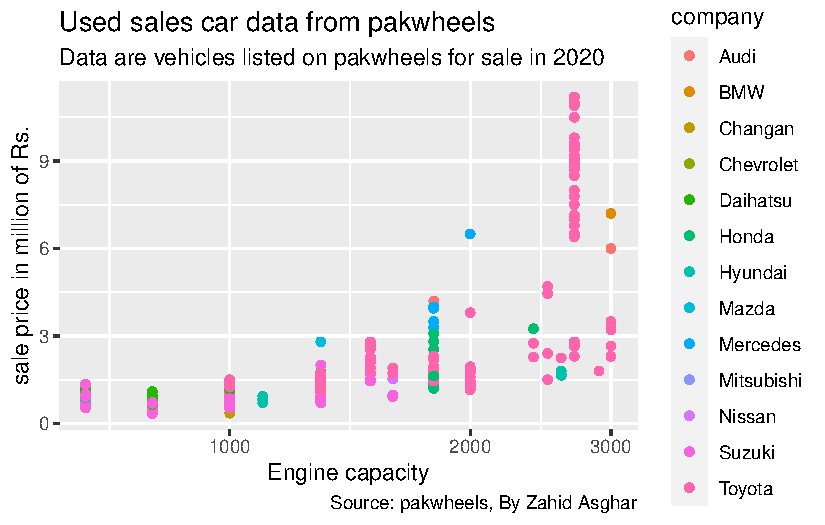
\includegraphics[width=17.1875in,height=\textheight]{pakwheels_files/figure-pdf/unnamed-chunk-26-1.pdf}

}

\end{figure}

If you just want to highlight the relationship between gbp per capita
and life Expectancy you've probably done most of the work now. However,
it is a good practice to highlight a few interesting dots in this chart
to give more insight to the plot:

\begin{Shaded}
\begin{Highlighting}[]

\CommentTok{\#| eval: false}
\CommentTok{\#tmp \textless{}{-} pkw \%\textgreater{}\%}
 \CommentTok{\#mutate(}
  \CommentTok{\# annotation = case\_when(}
   \CommentTok{\# hp \textless{} 2000 \& price \textless{} 700000 \textasciitilde{} "yes",}
    \CommentTok{\#price \textless{} 3000000 \textasciitilde{} "yes",}
     \CommentTok{\#Mileage \textgreater{} 15000 \textasciitilde{} "yes"}
    \CommentTok{\#)}
\CommentTok{\#) \%\textgreater{}\% mutate(Mileage=Mileage/10000)}
 \CommentTok{\# arrange(desc(price)) }

\CommentTok{\# Plot}
\CommentTok{\#ggplot( tmp, aes(x=hp, y=price, size =Mileage , color = company)) +}
 \CommentTok{\#   geom\_point(alpha=0.7) +}
  \CommentTok{\#  scale\_size(range = c(1.4, 19), name="Price in Million of Rupees") +}
   \CommentTok{\# scale\_color\_viridis(discrete=TRUE) +}
    \CommentTok{\#theme\_ipsum() +}
    \CommentTok{\#theme(legend.position="none") +}
    \CommentTok{\#geom\_text\_repel(data=tmp \%\textgreater{}\% filter(annotation=="yes"), aes(label=company), size=4 )}
\end{Highlighting}
\end{Shaded}

\hypertarget{section-2}{%
\subsection{}\label{section-2}}

\begin{Shaded}
\begin{Highlighting}[]
\DocumentationTok{\#\#This is a table of data about a large number of countries, each observed over several years. Let\textquotesingle{}s make a scatterplot with it.}
\CommentTok{\#| eval: false}
\NormalTok{P}\OtherTok{\textless{}{-}}\FunctionTok{ggplot}\NormalTok{(}\AttributeTok{data=}\NormalTok{pkw,}\AttributeTok{mapping =} \FunctionTok{aes}\NormalTok{(}\AttributeTok{x=}\NormalTok{hp,}\AttributeTok{y=}\NormalTok{price))  }

\NormalTok{P}\SpecialCharTok{+}\FunctionTok{geom\_point}\NormalTok{()}\SpecialCharTok{+}\FunctionTok{geom\_smooth}\NormalTok{()}
\end{Highlighting}
\end{Shaded}

\begin{figure}[H]

{\centering 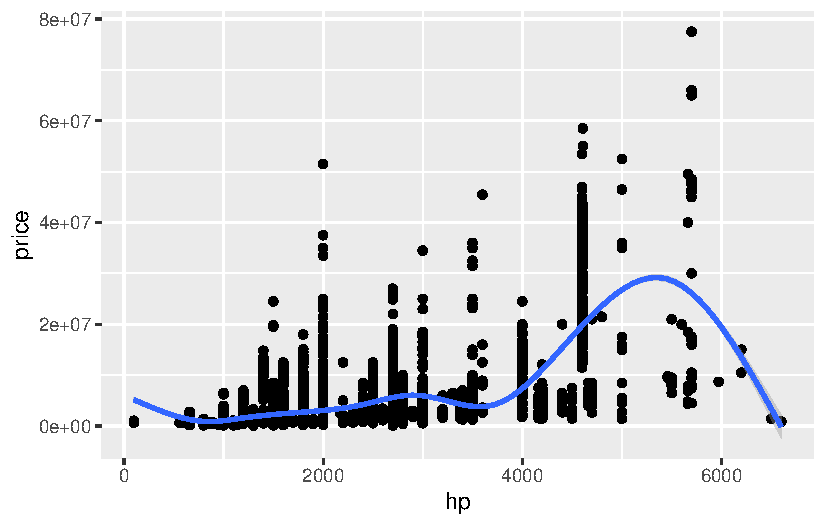
\includegraphics[width=17.1875in,height=\textheight]{pakwheels_files/figure-pdf/unnamed-chunk-29-1.pdf}

}

\end{figure}

\begin{Shaded}
\begin{Highlighting}[]

\NormalTok{P}\SpecialCharTok{+}\FunctionTok{geom\_point}\NormalTok{()}\SpecialCharTok{+}\FunctionTok{geom\_smooth}\NormalTok{(}\AttributeTok{method =} \StringTok{"lm"}\NormalTok{)}
\end{Highlighting}
\end{Shaded}

\begin{figure}[H]

{\centering 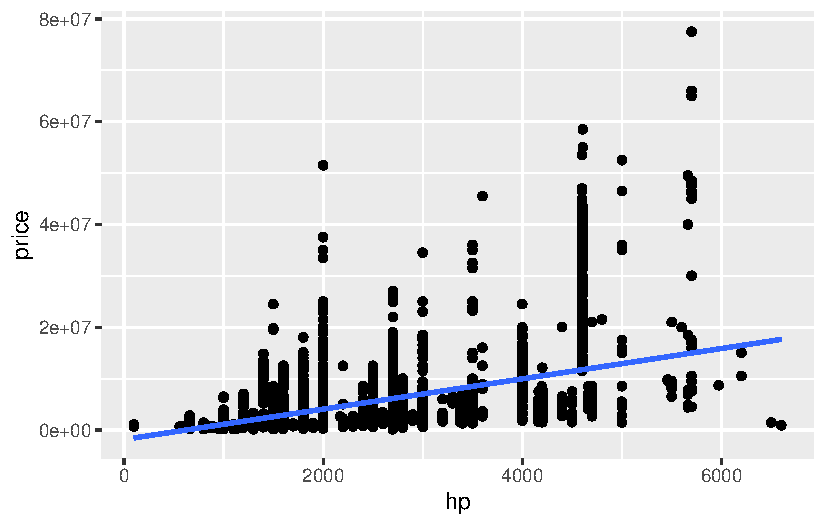
\includegraphics[width=17.1875in,height=\textheight]{pakwheels_files/figure-pdf/unnamed-chunk-29-2.pdf}

}

\end{figure}

\begin{Shaded}
\begin{Highlighting}[]

\NormalTok{P}\SpecialCharTok{+}\FunctionTok{geom\_point}\NormalTok{()}\SpecialCharTok{+}\FunctionTok{geom\_smooth}\NormalTok{(}\AttributeTok{method =} \StringTok{"gam"}\NormalTok{)}\SpecialCharTok{+}\FunctionTok{scale\_x\_log10}\NormalTok{()}
\end{Highlighting}
\end{Shaded}

\begin{figure}[H]

{\centering 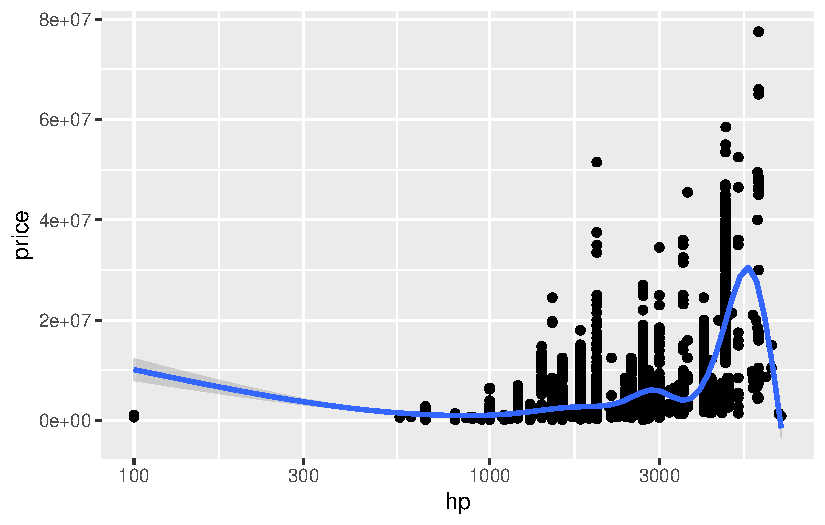
\includegraphics[width=17.1875in,height=\textheight]{pakwheels_files/figure-pdf/unnamed-chunk-29-3.pdf}

}

\end{figure}

\begin{Shaded}
\begin{Highlighting}[]


\NormalTok{P}\SpecialCharTok{+}\FunctionTok{geom\_point}\NormalTok{()}\SpecialCharTok{+}\FunctionTok{geom\_smooth}\NormalTok{(}\AttributeTok{method =} \StringTok{"gam"}\NormalTok{)}\SpecialCharTok{+}\FunctionTok{scale\_x\_log10}\NormalTok{(}\AttributeTok{labels=}\NormalTok{scales}\SpecialCharTok{::}\NormalTok{dollar)}
\end{Highlighting}
\end{Shaded}

\begin{figure}[H]

{\centering 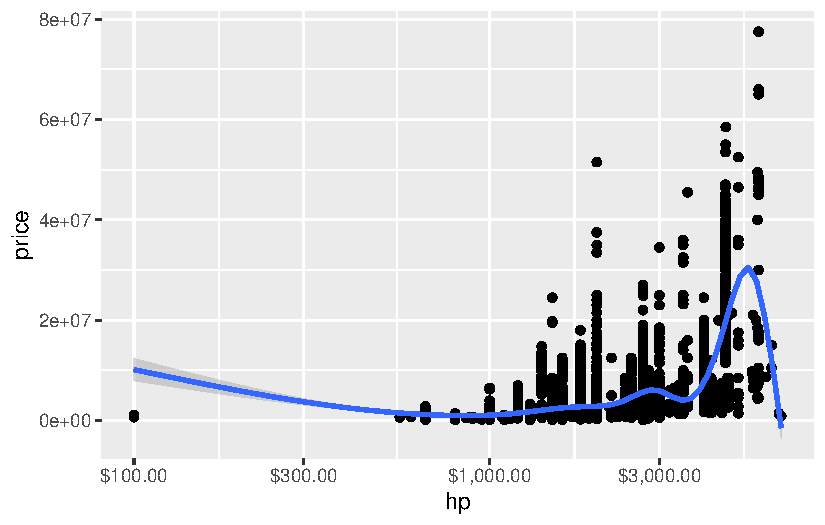
\includegraphics[width=17.1875in,height=\textheight]{pakwheels_files/figure-pdf/unnamed-chunk-29-4.pdf}

}

\end{figure}

\begin{Shaded}
\begin{Highlighting}[]


\NormalTok{P}\OtherTok{\textless{}{-}}\FunctionTok{ggplot}\NormalTok{(}\AttributeTok{data=}\NormalTok{pkw,}\AttributeTok{mapping =} \FunctionTok{aes}\NormalTok{(hp,}\AttributeTok{y=}\FunctionTok{log}\NormalTok{(price),}\AttributeTok{color=}\StringTok{"purple"}\NormalTok{))}
\NormalTok{P}\SpecialCharTok{+}\FunctionTok{geom\_point}\NormalTok{()}\SpecialCharTok{+}\FunctionTok{geom\_smooth}\NormalTok{(}\AttributeTok{method =} \StringTok{"loess"}\NormalTok{)}\SpecialCharTok{+}\FunctionTok{scale\_x\_log10}\NormalTok{()}
\end{Highlighting}
\end{Shaded}

\begin{figure}[H]

{\centering 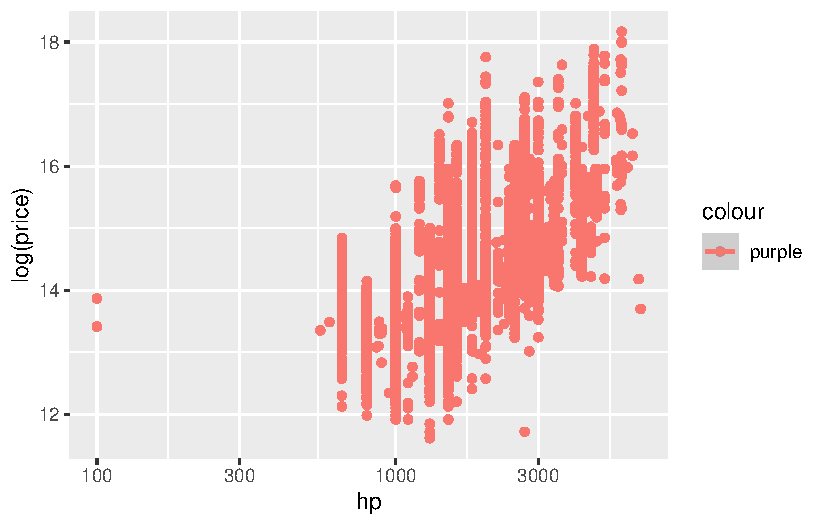
\includegraphics[width=17.1875in,height=\textheight]{pakwheels_files/figure-pdf/unnamed-chunk-29-5.pdf}

}

\end{figure}

\hypertarget{section-3}{%
\subsection{}\label{section-3}}

\begin{Shaded}
\begin{Highlighting}[]
\DocumentationTok{\#\#aes() is for variables}
\NormalTok{P}\OtherTok{\textless{}{-}}\FunctionTok{ggplot}\NormalTok{(}\AttributeTok{data=}\NormalTok{pkw,}\AttributeTok{mapping =} \FunctionTok{aes}\NormalTok{(hp,}\AttributeTok{y=}\FunctionTok{log}\NormalTok{(price)))}
\NormalTok{P}\SpecialCharTok{+}\FunctionTok{geom\_point}\NormalTok{(}\AttributeTok{color=}\StringTok{"purple"}\NormalTok{)}\SpecialCharTok{+}\FunctionTok{geom\_smooth}\NormalTok{(}\AttributeTok{method =} \StringTok{"loess"}\NormalTok{)}\SpecialCharTok{+}\FunctionTok{scale\_x\_log10}\NormalTok{()}
\end{Highlighting}
\end{Shaded}

\hypertarget{section-4}{%
\subsection{}\label{section-4}}

\begin{Shaded}
\begin{Highlighting}[]
\NormalTok{P}\OtherTok{\textless{}{-}}\FunctionTok{ggplot}\NormalTok{(}\AttributeTok{data=}\NormalTok{pkw,}\AttributeTok{mapping =} \FunctionTok{aes}\NormalTok{(hp,}\AttributeTok{y=}\NormalTok{price))}
\NormalTok{P}\SpecialCharTok{+}\FunctionTok{geom\_point}\NormalTok{(}\AttributeTok{alpha=}\FloatTok{0.3}\NormalTok{)}\SpecialCharTok{+}
  \FunctionTok{geom\_smooth}\NormalTok{(}\AttributeTok{color=}\StringTok{"orange"}\NormalTok{,}\AttributeTok{se=}\ConstantTok{FALSE}\NormalTok{,}\AttributeTok{size=}\DecValTok{5}\NormalTok{,}\AttributeTok{method =} \StringTok{"lm"}\NormalTok{)}\SpecialCharTok{+}
  \FunctionTok{scale\_x\_log10}\NormalTok{()}
\end{Highlighting}
\end{Shaded}

\begin{figure}[H]

{\centering 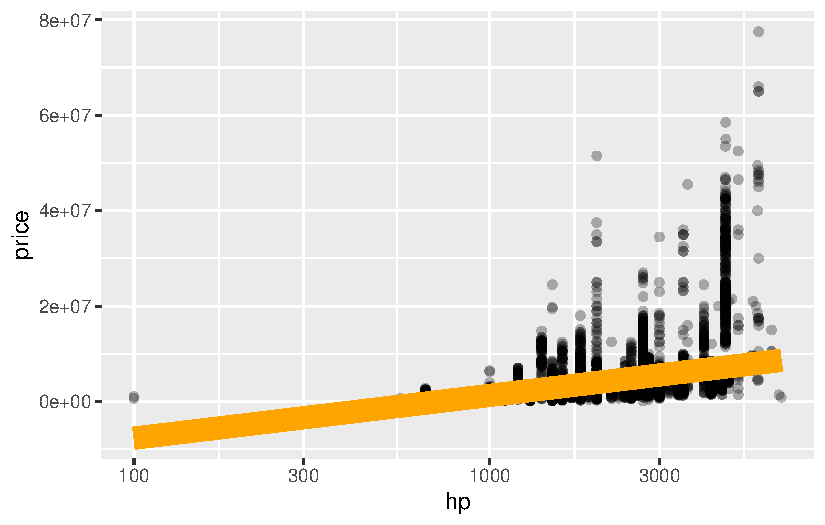
\includegraphics[width=17.1875in,height=\textheight]{pakwheels_files/figure-pdf/unnamed-chunk-31-1.pdf}

}

\end{figure}

\hypertarget{section-5}{%
\subsection{}\label{section-5}}

\begin{Shaded}
\begin{Highlighting}[]
\CommentTok{\#With proper title}
\NormalTok{P}\OtherTok{\textless{}{-}}\FunctionTok{ggplot}\NormalTok{(}\AttributeTok{data=}\NormalTok{pkw,}\AttributeTok{mapping =} \FunctionTok{aes}\NormalTok{(hp,}\AttributeTok{y=}\FunctionTok{log}\NormalTok{(price)))}
\NormalTok{P}\SpecialCharTok{+}\FunctionTok{geom\_point}\NormalTok{(}\AttributeTok{alpha=}\FloatTok{0.3}\NormalTok{)}\SpecialCharTok{+}
  \FunctionTok{geom\_smooth}\NormalTok{(}\AttributeTok{method =} \StringTok{"gam"}\NormalTok{)}\SpecialCharTok{+}
  \FunctionTok{scale\_y\_log10}\NormalTok{()}\SpecialCharTok{+}
  \FunctionTok{labs}\NormalTok{(}\AttributeTok{x =} \StringTok{"engine capacity"}\NormalTok{, }\AttributeTok{y =} \StringTok{"price of a car for sale"}\NormalTok{,}
       \AttributeTok{title =} \StringTok{"pakwheels car sale data"}\NormalTok{,}
       \AttributeTok{subtitle =} \StringTok{"Data points are company{-}years"}\NormalTok{,}
       \AttributeTok{caption =} \StringTok{"Source: pakwheels."}\NormalTok{)}
\end{Highlighting}
\end{Shaded}

\begin{figure}[H]

{\centering 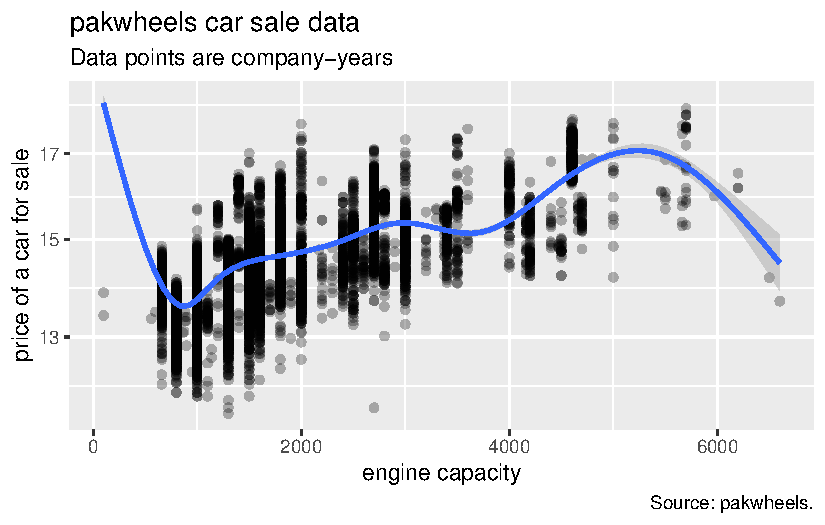
\includegraphics[width=17.1875in,height=\textheight]{pakwheels_files/figure-pdf/unnamed-chunk-32-1.pdf}

}

\end{figure}

\hypertarget{section-6}{%
\subsection{}\label{section-6}}

\begin{Shaded}
\begin{Highlighting}[]
\DocumentationTok{\#\#Continent wise}
\CommentTok{\#| eval: false}

\NormalTok{p }\OtherTok{\textless{}{-}} \FunctionTok{ggplot}\NormalTok{(}\AttributeTok{data =}\NormalTok{ pkw,}
            \AttributeTok{mapping =} \FunctionTok{aes}\NormalTok{(}\AttributeTok{x =}\NormalTok{ hp,}
                          \AttributeTok{y =}\NormalTok{ price,}
                          \AttributeTok{color =}\NormalTok{ company))}
\NormalTok{p }\SpecialCharTok{+} \FunctionTok{geom\_point}\NormalTok{() }\SpecialCharTok{+}
  \FunctionTok{geom\_smooth}\NormalTok{(}\AttributeTok{method =} \StringTok{"loess"}\NormalTok{) }\SpecialCharTok{+}
  \FunctionTok{scale\_x\_log10}\NormalTok{()}
\end{Highlighting}
\end{Shaded}

\begin{figure}[H]

{\centering 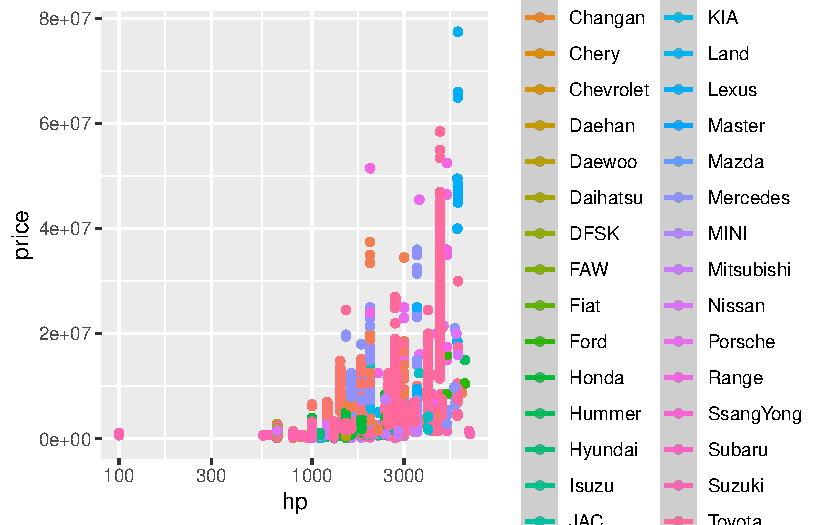
\includegraphics[width=17.1875in,height=\textheight]{pakwheels_files/figure-pdf/unnamed-chunk-33-1.pdf}

}

\end{figure}

\begin{Shaded}
\begin{Highlighting}[]
\NormalTok{p }\OtherTok{\textless{}{-}}\NormalTok{pkw}\SpecialCharTok{|\textgreater{}} \FunctionTok{filter}\NormalTok{(hp}\SpecialCharTok{\textgreater{}}\DecValTok{300}\NormalTok{)}\SpecialCharTok{|\textgreater{}} \FunctionTok{ggplot}\NormalTok{(}\FunctionTok{aes}\NormalTok{(}\AttributeTok{x =}\NormalTok{ hp,}
                          \AttributeTok{y =}\NormalTok{ price,}
                          \AttributeTok{color =}\NormalTok{ Assembly,}
                          \AttributeTok{fill =}\NormalTok{ Assembly))}
\NormalTok{p }\SpecialCharTok{+} \FunctionTok{geom\_point}\NormalTok{() }\SpecialCharTok{+}
  \FunctionTok{geom\_smooth}\NormalTok{(}\AttributeTok{method =} \StringTok{"loess"}\NormalTok{) }\SpecialCharTok{+}
  \FunctionTok{scale\_x\_log10}\NormalTok{()}\SpecialCharTok{+}\FunctionTok{scale\_y\_continuous}\NormalTok{()}
\end{Highlighting}
\end{Shaded}

\begin{Shaded}
\begin{Highlighting}[]
\DocumentationTok{\#\#Aesthetics can be mapped per geom}
\CommentTok{\#| eval: false}
\NormalTok{p }\OtherTok{\textless{}{-}}\NormalTok{pkw}\SpecialCharTok{|\textgreater{}}\FunctionTok{filter}\NormalTok{(hp}\SpecialCharTok{\textgreater{}}\DecValTok{500}\NormalTok{)}\SpecialCharTok{|\textgreater{}} \FunctionTok{ggplot}\NormalTok{(}\FunctionTok{aes}\NormalTok{(}\AttributeTok{x =}\NormalTok{ hp, }\AttributeTok{y =} \FunctionTok{log}\NormalTok{(price)))}
\NormalTok{p }\SpecialCharTok{+} \FunctionTok{geom\_point}\NormalTok{(}\AttributeTok{mapping =} \FunctionTok{aes}\NormalTok{(}\AttributeTok{color =}\NormalTok{ company)) }\SpecialCharTok{+}
  \FunctionTok{geom\_smooth}\NormalTok{(}\AttributeTok{method =} \StringTok{"loess"}\NormalTok{) }\SpecialCharTok{+}\FunctionTok{scale\_y\_log10}\NormalTok{()}\SpecialCharTok{+}
  \FunctionTok{scale\_x\_log10}\NormalTok{()}
\end{Highlighting}
\end{Shaded}

\begin{figure}[H]

{\centering 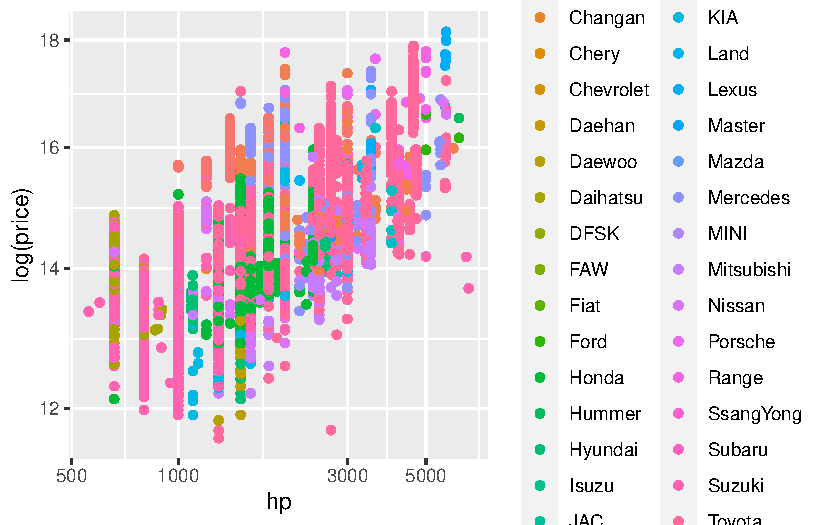
\includegraphics[width=17.1875in,height=\textheight]{pakwheels_files/figure-pdf/unnamed-chunk-35-1.pdf}

}

\end{figure}

\begin{Shaded}
\begin{Highlighting}[]


\NormalTok{p }\SpecialCharTok{+} \FunctionTok{geom\_point}\NormalTok{(}\AttributeTok{mapping =} \FunctionTok{aes}\NormalTok{(}\AttributeTok{color =}\NormalTok{ company)) }\SpecialCharTok{+}
  \FunctionTok{scale\_x\_log10}\NormalTok{()}\SpecialCharTok{+}\FunctionTok{scale\_y\_log10}\NormalTok{()}
\end{Highlighting}
\end{Shaded}

\begin{figure}[H]

{\centering 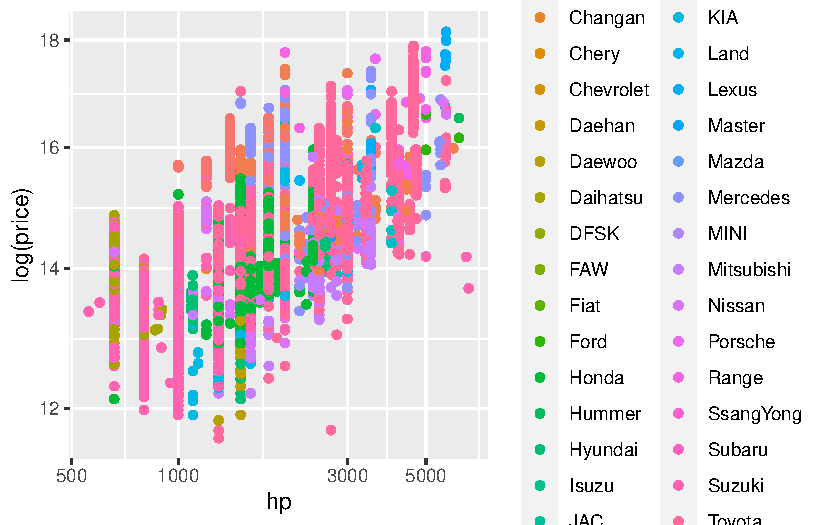
\includegraphics[width=17.1875in,height=\textheight]{pakwheels_files/figure-pdf/unnamed-chunk-35-2.pdf}

}

\end{figure}

\hypertarget{bar-plot}{%
\subsection{Bar plot}\label{bar-plot}}

\begin{Shaded}
\begin{Highlighting}[]
\NormalTok{manufacturers }\OtherTok{\textless{}{-}}\NormalTok{ pkw }\SpecialCharTok{|\textgreater{}} 
  \FunctionTok{count}\NormalTok{(company, }\AttributeTok{sort =} \ConstantTok{TRUE}\NormalTok{) }\SpecialCharTok{|\textgreater{}} 
  \FunctionTok{mutate}\NormalTok{(}
    \AttributeTok{manufacturer =} \FunctionTok{str\_to\_title}\NormalTok{(company),}
    \AttributeTok{manufacturer =} \FunctionTok{fct\_reorder}\NormalTok{(company, n) }
\NormalTok{  )}\SpecialCharTok{|\textgreater{}}\FunctionTok{na.omit}\NormalTok{()}
\NormalTok{manufacturers }\SpecialCharTok{|\textgreater{}} \FunctionTok{filter}\NormalTok{(n}\SpecialCharTok{\textgreater{}}\DecValTok{100}\NormalTok{)}\SpecialCharTok{|\textgreater{}}
  \FunctionTok{ggplot}\NormalTok{(}\FunctionTok{aes}\NormalTok{(}\AttributeTok{y =}\NormalTok{ manufacturer, }\AttributeTok{x =}\NormalTok{ n)) }\SpecialCharTok{+}
  \FunctionTok{geom\_col}\NormalTok{(}\AttributeTok{fill =} \StringTok{\textquotesingle{}dodgerblue4\textquotesingle{}}\NormalTok{) }\SpecialCharTok{+}
  \FunctionTok{theme\_minimal}\NormalTok{() }\SpecialCharTok{+}
  \FunctionTok{scale\_x\_continuous}\NormalTok{(}
    \AttributeTok{expand =} \FunctionTok{expansion}\NormalTok{(}\AttributeTok{mult =} \FunctionTok{c}\NormalTok{(}\DecValTok{0}\NormalTok{, }\FloatTok{0.05}\NormalTok{))}
\NormalTok{  ) }\SpecialCharTok{+}
  \FunctionTok{labs}\NormalTok{(}
    \AttributeTok{x =} \FunctionTok{element\_blank}\NormalTok{(), }
    \AttributeTok{y =} \FunctionTok{element\_blank}\NormalTok{(),}
    \AttributeTok{title =} \StringTok{\textquotesingle{}Number of vehicles in the Pakwheels data set\textquotesingle{}}\NormalTok{,}
    \AttributeTok{subtitle =} \StringTok{"At least 100 vehicles should be in the data to be included in graph"}\NormalTok{,}
    \AttributeTok{caption =} \StringTok{"Source: Pakwheels| Zahid Asghar "}
\NormalTok{  ) }\SpecialCharTok{+}
  \FunctionTok{theme}\NormalTok{(}
    \AttributeTok{panel.grid.major.y =} \FunctionTok{element\_blank}\NormalTok{()}
\NormalTok{  )}
\end{Highlighting}
\end{Shaded}

\begin{figure}[H]

{\centering 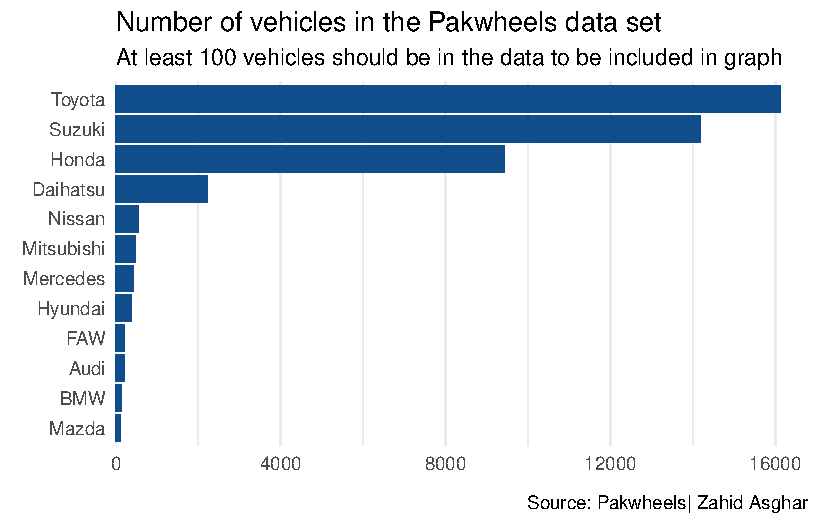
\includegraphics[width=17.1875in,height=\textheight]{pakwheels_files/figure-pdf/unnamed-chunk-36-1.pdf}

}

\end{figure}

\hypertarget{lollipop-chart}{%
\subsection{Lollipop chart}\label{lollipop-chart}}

\begin{Shaded}
\begin{Highlighting}[]
\NormalTok{manufacturers }\SpecialCharTok{|\textgreater{}} \FunctionTok{filter}\NormalTok{(n}\SpecialCharTok{\textgreater{}}\DecValTok{100}\NormalTok{)}\SpecialCharTok{|\textgreater{}}
  \FunctionTok{ggplot}\NormalTok{(}\FunctionTok{aes}\NormalTok{(}\AttributeTok{y =}\NormalTok{ manufacturer, }\AttributeTok{x =}\NormalTok{ n)) }\SpecialCharTok{+}
  \FunctionTok{geom\_point}\NormalTok{(}\AttributeTok{col =} \StringTok{\textquotesingle{}dodgerblue4\textquotesingle{}}\NormalTok{, }\AttributeTok{size =} \DecValTok{5}\NormalTok{) }\SpecialCharTok{+}
  \FunctionTok{geom\_segment}\NormalTok{(}
    \FunctionTok{aes}\NormalTok{(}\AttributeTok{x =} \DecValTok{0}\NormalTok{, }\AttributeTok{xend =}\NormalTok{ n, }\AttributeTok{y =}\NormalTok{ manufacturer, }\AttributeTok{yend =}\NormalTok{ manufacturer),}
    \AttributeTok{linewidth =} \FloatTok{1.5}\NormalTok{,}
    \AttributeTok{col =} \StringTok{\textquotesingle{}dodgerblue4\textquotesingle{}}
\NormalTok{  ) }\SpecialCharTok{+}
  \FunctionTok{theme\_minimal}\NormalTok{() }\SpecialCharTok{+}
  \FunctionTok{scale\_x\_continuous}\NormalTok{(}
    \AttributeTok{expand =} \FunctionTok{expansion}\NormalTok{(}\AttributeTok{mult =} \FunctionTok{c}\NormalTok{(}\DecValTok{0}\NormalTok{, }\FloatTok{0.05}\NormalTok{))}
\NormalTok{  ) }\SpecialCharTok{+}
  \FunctionTok{labs}\NormalTok{(}
    \AttributeTok{x =} \FunctionTok{element\_blank}\NormalTok{(), }
    \AttributeTok{y =} \FunctionTok{element\_blank}\NormalTok{(),}
    \AttributeTok{title =} \StringTok{\textquotesingle{}Number of vehicles in the Pakwheels data set\textquotesingle{}}\NormalTok{,}
    \AttributeTok{subtitle =} \StringTok{"At least 100 vehicles should be in the data to be included in graph"}\NormalTok{,}
    \AttributeTok{caption =} \StringTok{"Source: Pakwheels| Zahid Asghar "}
\NormalTok{  ) }\SpecialCharTok{+}
  \FunctionTok{theme}\NormalTok{(}
    \AttributeTok{panel.grid.major.y =} \FunctionTok{element\_blank}\NormalTok{()}
\NormalTok{  )}
\end{Highlighting}
\end{Shaded}

\begin{figure}[H]

{\centering 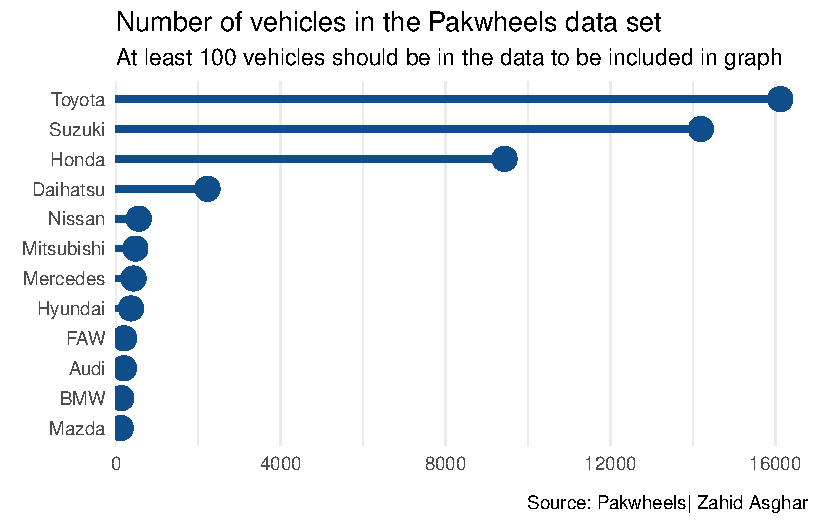
\includegraphics[width=17.1875in,height=\textheight]{pakwheels_files/figure-pdf/unnamed-chunk-37-1.pdf}

}

\end{figure}



\end{document}
